
\documentclass[fleqn,addpoints]{exam}

\usepackage{graphicx}
\usepackage{float}
\usepackage{amsmath}
\usepackage{cancel}
\usepackage{polynom}

\printanswers

\ifprintanswers \usepackage{2in1, lscape} \fi

\title{Math 115 Homework 3}
\date{October 12, 2010}

\begin{document}

\maketitle

\ifprintanswers
\else

\section{Key Points}
\subsection{Linear Equations and Functions}

\begin{itemize}

\item A linear equation/function is any equation/function of the form: $y = mx + b$ or $f(x) = mx + b$.  The graphs of linear
  equations are straight lines.  

\item $f(x) = mx + b$ is called the {\em slope-intercept} form of the line.  $m$ is the slope and $(0, b)$ is the y-intercept.

\item If you know two points on a line, you can figure out the line's slope using:
\[
  m = \frac{y_2-y_1}{x_2-x_1}
\]
It doesn't matter which point you put first, but you have to be consistent.  So this equation won't give the correct
slope since the points are subtracted in different orders in the numerator and denominator:
\[
  m \ne \frac{y_2-y_1}{x_1-x_2} (\text{ don't do this})
\]

\item The {\em point-slope} form of the equation of a line is: $y - y_1 = m(x - x_1)$.  $m$ is the slope and 
  $(x_1, y_1)$ is any point on the line.  Of course, there is more than one {\em point-slope} equation for the same
  line, since you can use any point on the line.

\item Two lines are parallel if and only if they have the same slope and different y-intercepts.

\item Two lines are perpendicular if and only if the slope of one line is the negative reciprocal of the slope of the other line.

\end{itemize}

\subsection{Transformations}

Transformations are things you do to a function to move it around or change its shape.  You can apply several
transformations to the same function to, for example, move it up and to the left while flipping it upside down.

\subsubsection{Rigid Transformation}

A {\em rigid transformation} is something you do to a function which causes its graph to move around on the x/y plane
without changing its shape.

Given a function, $f(x)$ and positive constant $c$:

\begin{itemize}

\item $g(x) = f(x) + c$;  $g(x)$ is $f(x)$ shifted c-units up.
\item $g(x) = f(x) - c$;  $g(x)$ is $f(x)$ shifted c-units down.
\item $g(x) = f(x+c)$;  $g(x)$ is $f(x)$ shifted c-units left.
\item $g(x) = f(x-c)$;  $g(x)$ is $f(x)$ shifted c-units right.
\item $g(x) = -f(x)$;  $g(x)$ is $f(x)$ reflected around the x-axis (flipped upside down).
\item $g(x) = f(-x)$;  $g(x)$ is $f(x)$ reflected around the y-axis (flipped left to right).

\end{itemize}

\subsubsection{Non-Rigid Transformation}

A {\em non-rigid transformation} is something you do to a function which causes it to stay in the same place but
change its shape.

Given a function, $f(x)$ and $c > 1$:

\begin{itemize}

\item $g(x) = c \cdot f(x)$;  $g(x)$ is $f(x)$ stretched vertically.
\item $g(x) = \dfrac{1}{c} \cdot f(x)$;  $g(x)$ is $f(x)$ stretched horizontally.

\end{itemize}

\subsection{Quadratic Equations}

\begin{itemize}

\item A quadratic function/equation is any function/equation of the form: $f(x) = ax^2 + bx + c$ or $y = ax^2 + bx + c$ ($a \neq 0$).  Graphs of
  quadratic equations are U-shaped curves called {\em parabolas}.

\item The standard form of a quadratic function is: $f(x) = a(x-h)^2 + k$.  $(h, k)$ is called the {\em vertex} and is the
  lowest (or highest, if $a$ is negative) point on the parabola.

\item To convert a function from $f(x) = ax^2+bx+c$ form to the standard form, you can use the {\em complete the square} technique.

\item For the function $f(x) = ax^2+bx+c$, the vertex is at $\left( -\dfrac{b}{2a}, \dfrac{4ac - b^2}{4a} \right)$.  

  If you are like me, you may find the formula for the y-coordinate hard to remember, so you might prefer: 
  $\left( - \dfrac{b}{2a}, f \left(- \dfrac{b}{2a} \right) \right)$.

\item You can find the solution to any quadratic equation in the form: $ax^2+bx+c=0$ using the quadratic formula:
\[
  x = \frac{-b \pm \sqrt{b^2-4ac}}{2a}
\]

\end{itemize}
\pagebreak

\fi

\section{Homework}

\subsection{From the Book}

Read sections 1.7 and 1.8.
 
\begin{itemize}
  \item pp. 54-55: 1, 5-6, 9-16, 18, 21
  \item pp. 65-66: 1, 3, 5, 6, 19, 21, 23, 30
\end{itemize}

\ifprintanswers

\section{Pages 54-55}
\begin{itemize}

\item[1]
\begin{itemize}

\item[a]
slope:
\[
  m = \frac{2-0}{1-0} = 2
\]

equation:
\begin{align*}
  y - 0 &= 2(x-0) \\
  y &= 2x \\
\end{align*}

graph:
\begin{figure}[H]
  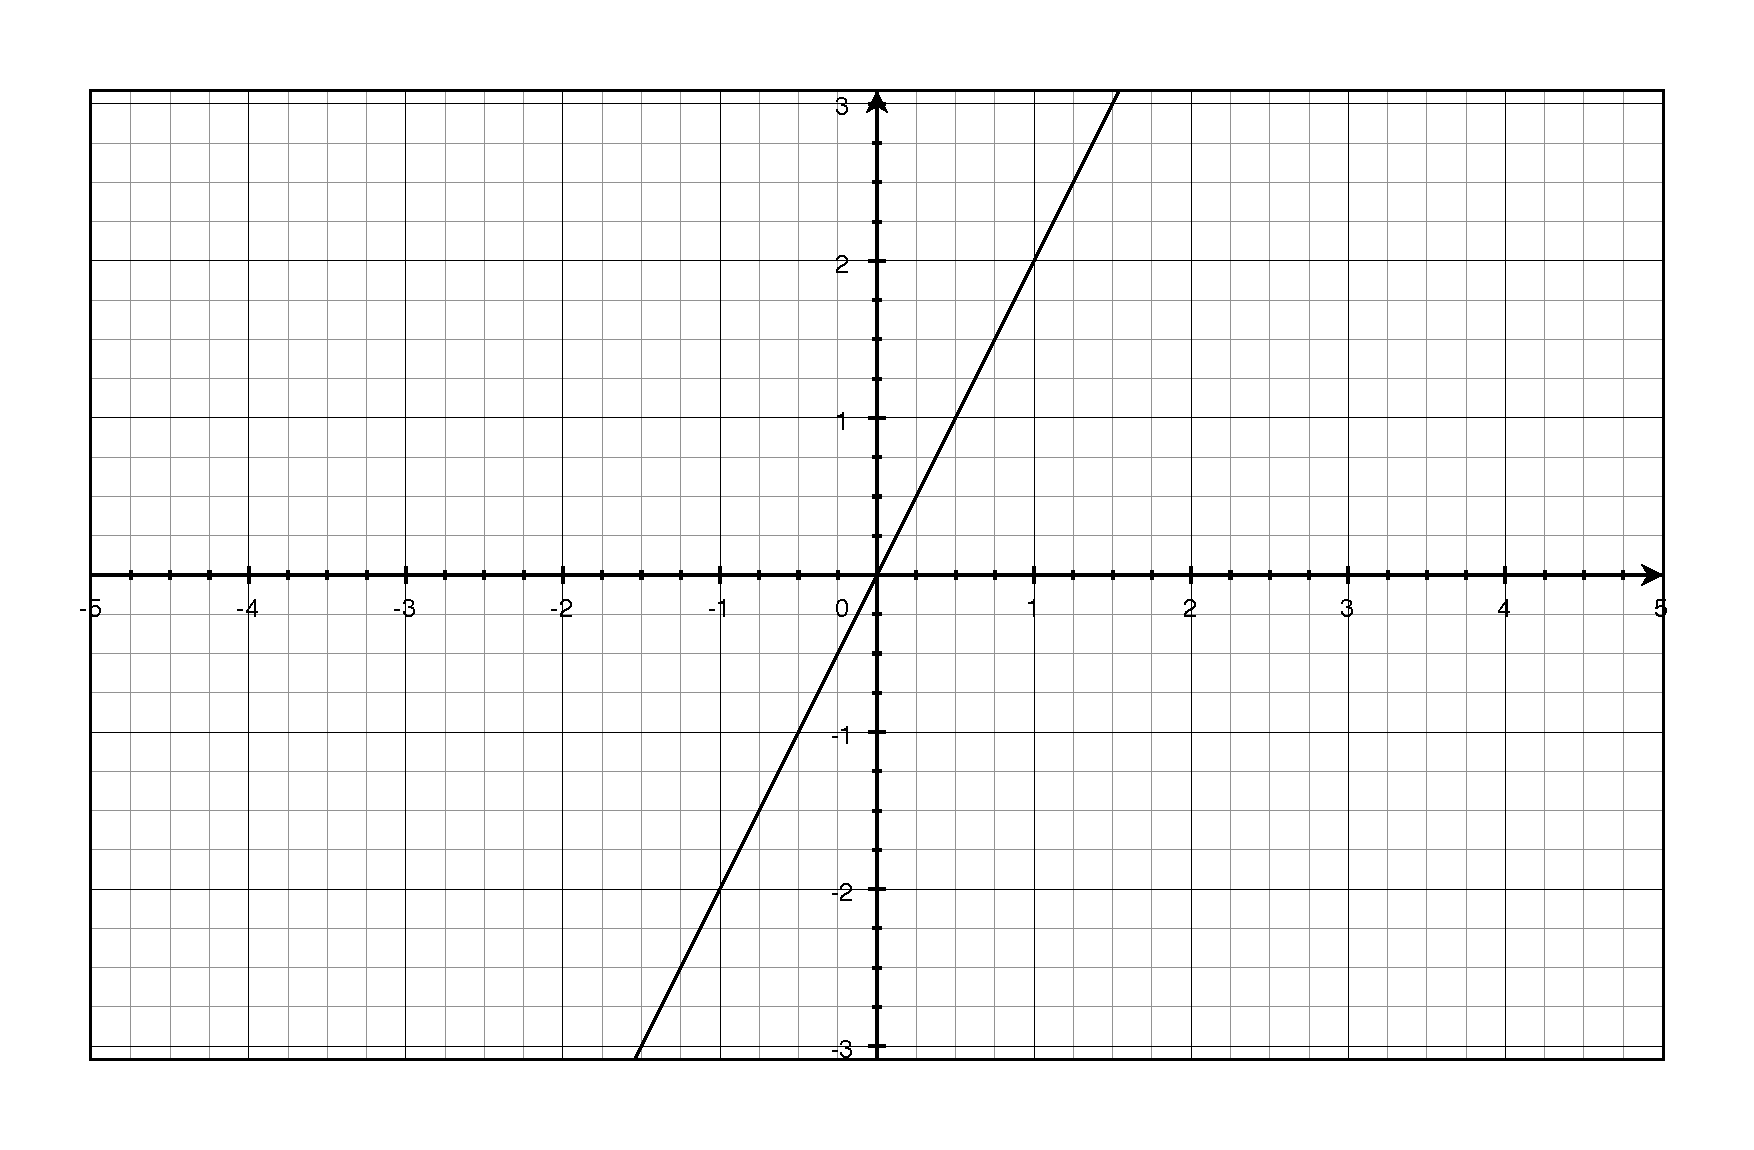
\includegraphics[width=7cm,height=5cm]{1.7-1a.eps}
\end{figure}

\item[b]
slope:
\[
  m = \frac{2- (-2)}{1-3} = \frac{4}{-2} = -2
\]

equation:
\begin{align*}
  y - 2 &= -2(x-1) \\
  y - 2 &= -2x + 2 \\
  y &= -2x + 4 \\
\end{align*}

graph:
\begin{figure}[H]
  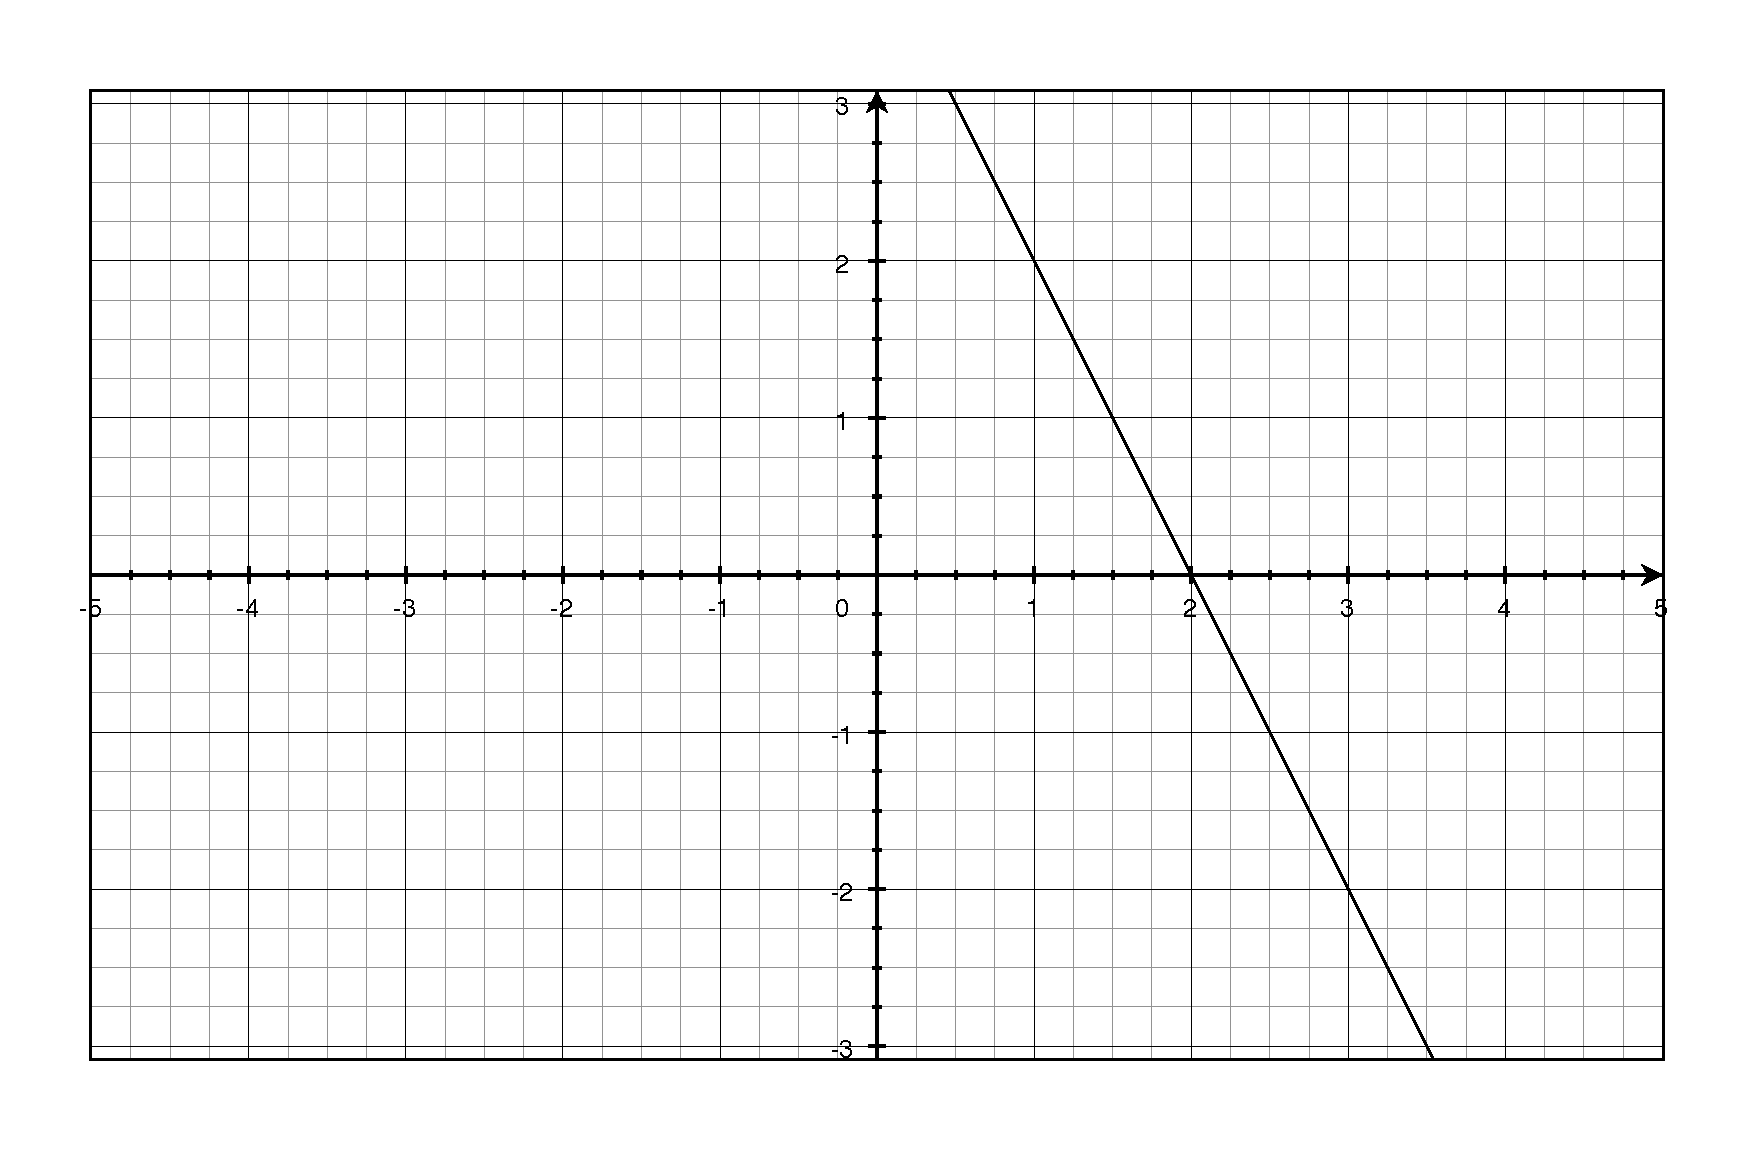
\includegraphics[width=7cm,height=5cm]{1.7-1b.eps}
\end{figure}

\item[c]
slope:
\[
  m = \frac{1- (-3)}{5-1} = \frac{4}{4} = 1
\]

equation:
\begin{align*}
  y - (-3) &= x-1 \\
  y + 3 &= x-1 \\
  y &= x-4 \\
\end{align*}

graph:
\begin{figure}[H]
  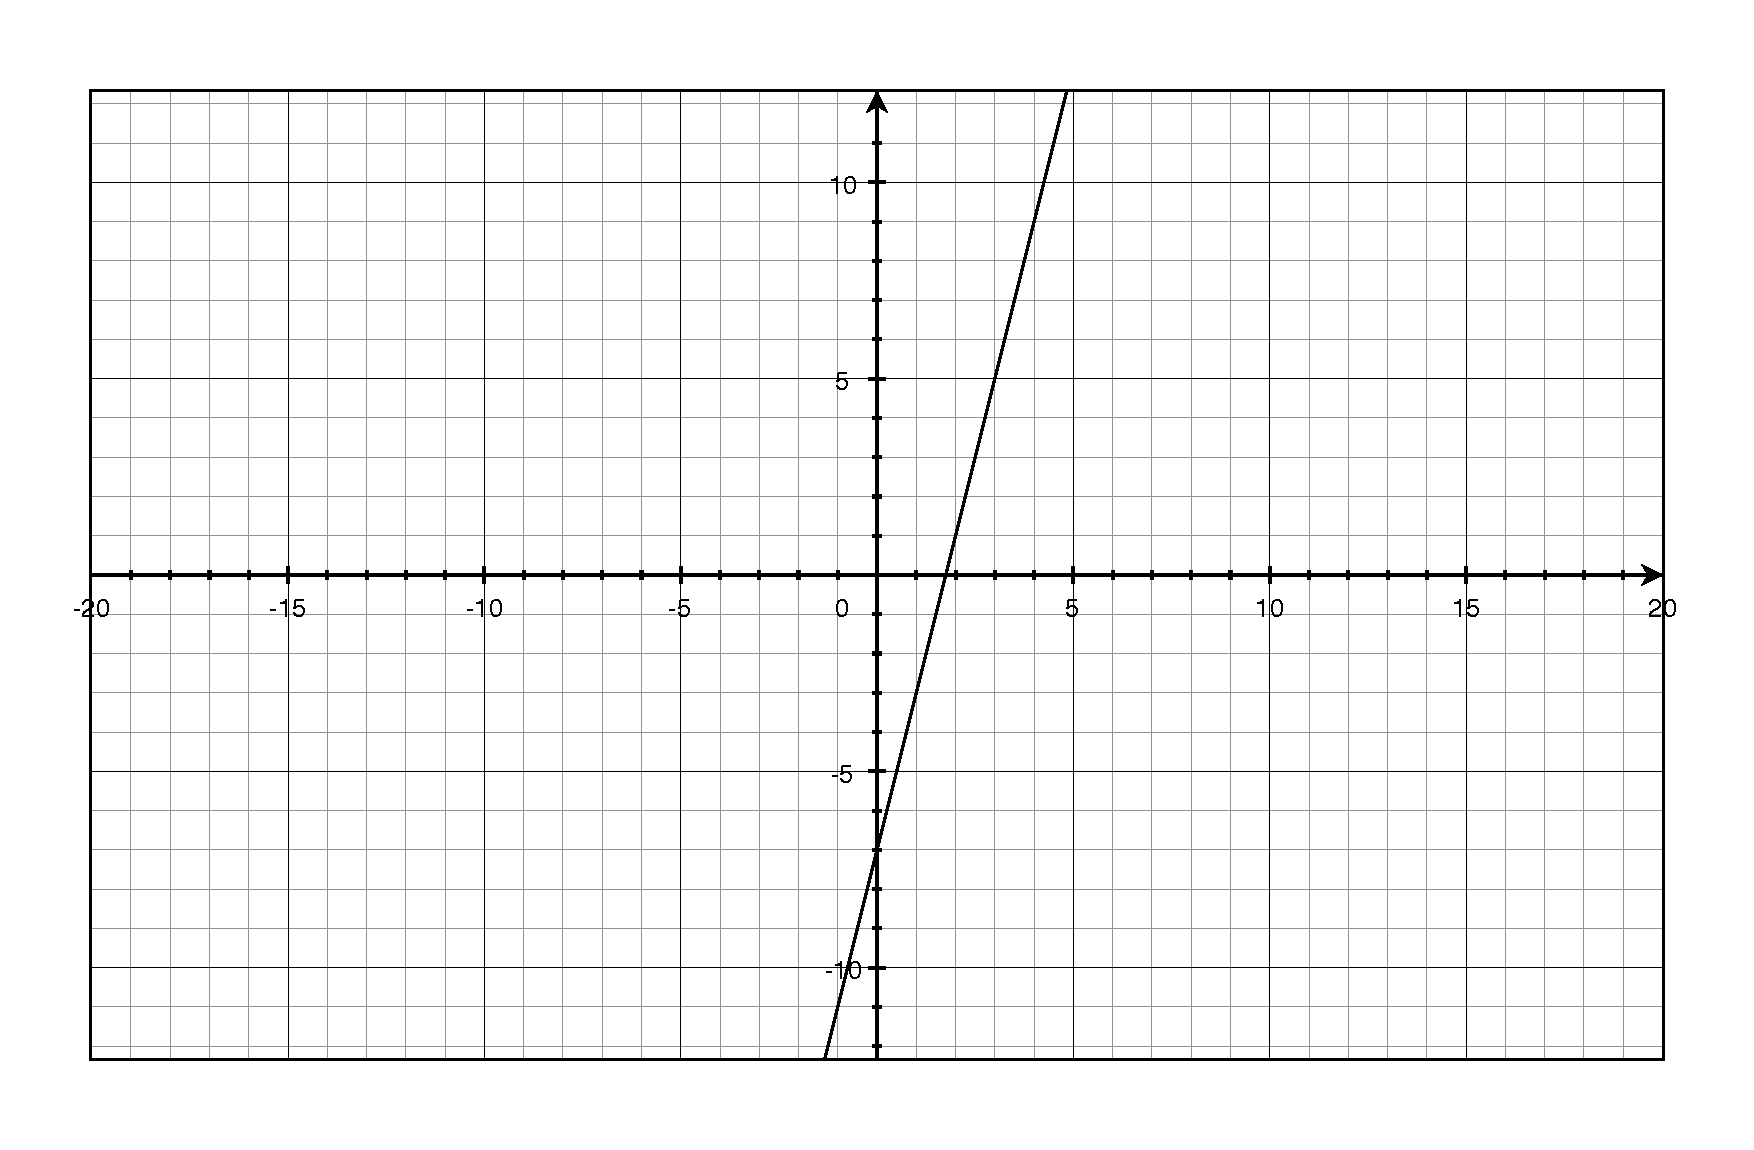
\includegraphics[width=7cm,height=5cm]{1.7-1c.eps}
\end{figure}


\item[d]
slope:
\[
  m = \frac{-1-3}{-5 - (-1)} = \frac{-4}{-4} = 1
\]

equation:
\begin{align*}
  y - 3 &= x - (-1) \\
  y - 3 &= x +1 \\
  y &= x + 4 \\
\end{align*}

graph:
\begin{figure}[H]
  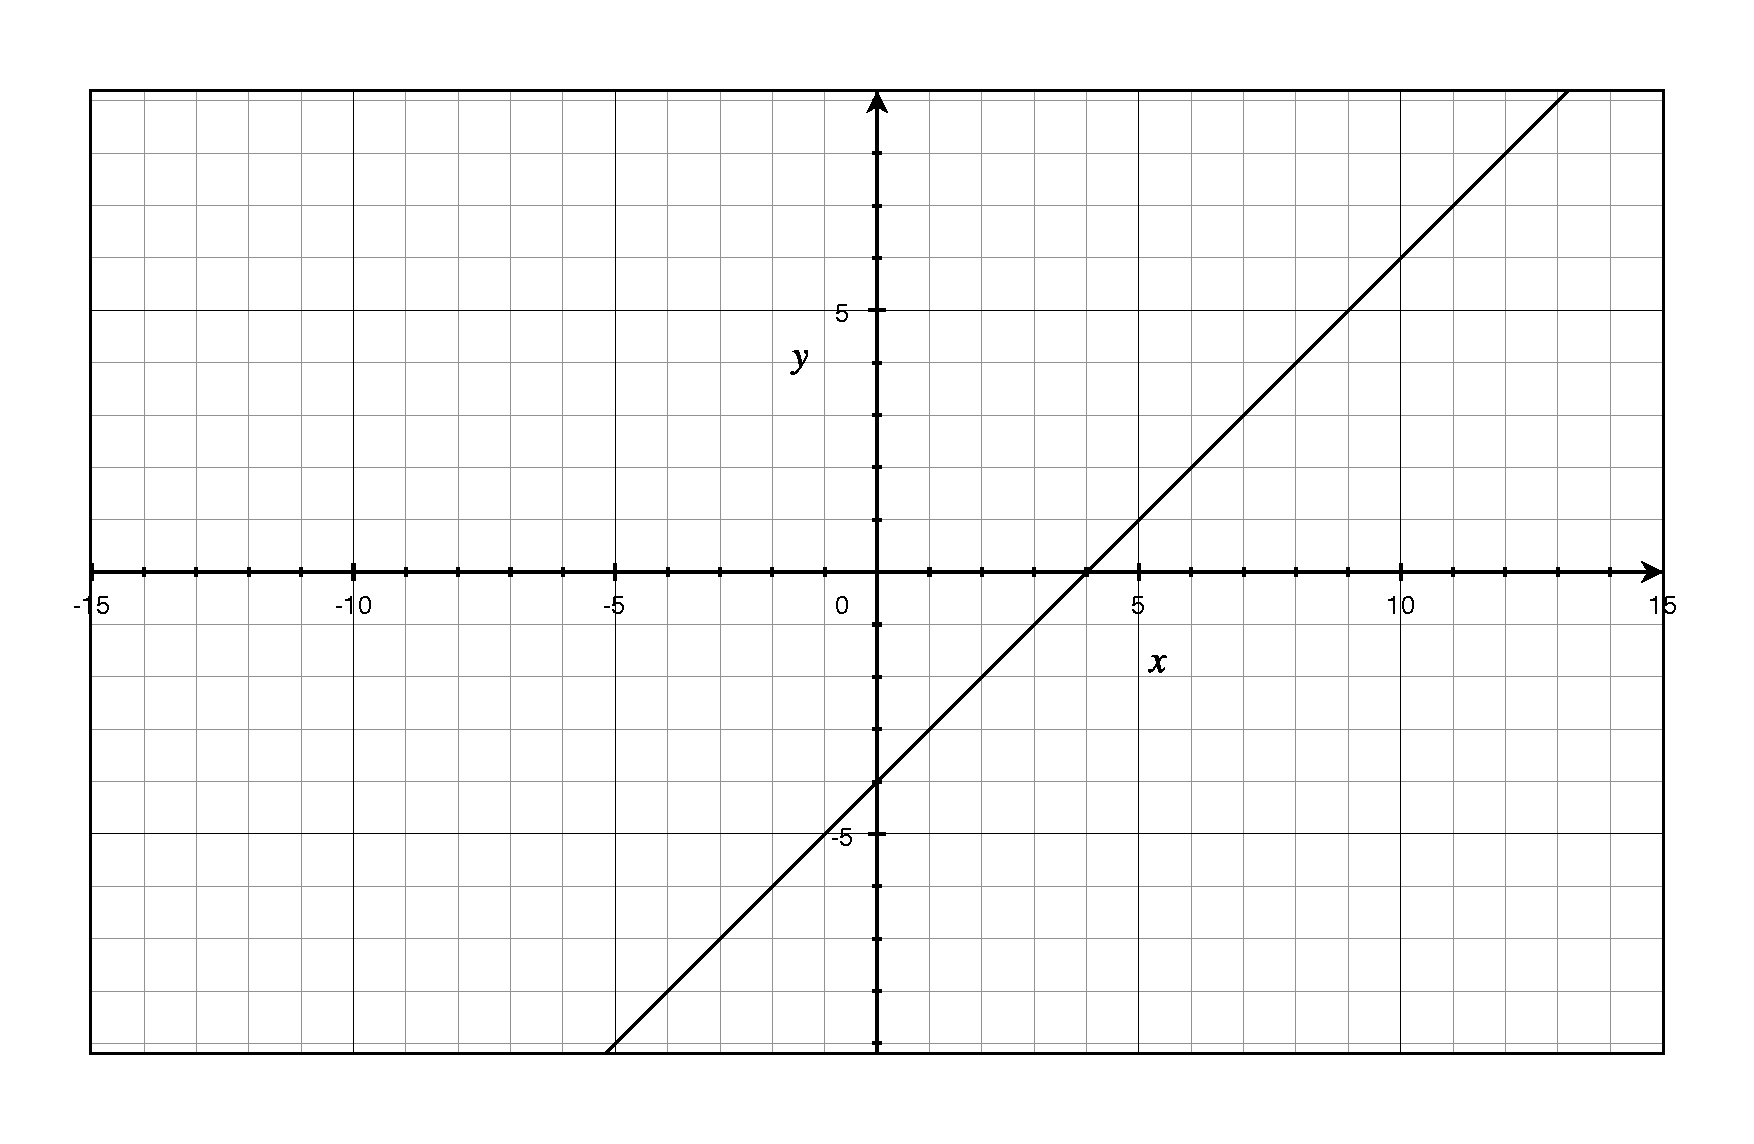
\includegraphics[width=7cm,height=5cm]{1.7-1d.eps}
\end{figure}

\end{itemize}

\item[5]

parallel:
\begin{align*}
  y-0 &= 2(x-0) \\
  y &= 2x \\
\end{align*}

perpendicular
\begin{align*}
  y-0 &= -\frac{1}{2}(x-0) \\
  y   &= -\frac{1}{2}x \\
\end{align*}

\item[6]

parallel:
\begin{align*}
  y-2 &= 3(x-1) \\
  y-2 &= 3x-3 \\
  y &= 3x-1 \\
\end{align*}

perpendicular
\begin{align*}
  y-2 &= -\frac{1}{3} (x-1) \\
  y-2 &= -\frac{1}{3} x + \frac{1}{3} \\
  y &= -\frac{1}{3} x + \frac{7}{3} \\
\end{align*}

\item[9]

\begin{align*}
  3 &= \frac{y - (-2)}{x-1} \\
  y + 2 &= 3x - 3 \\
  y &= 3x - 5 \\
\end{align*}

\item[10]
\begin{align*}
  y + 3 &= -2(x + 1) \\
  y + 3 &= -2x - 2 \\
  y  &= -2x - 5 \\
\end{align*}

\item[11]
\[
  y = -x + 2
\]

\item[12]
The line passes through $(2, 0)$ and $(0, 4)$.

First find the slope:
\[
  m = \frac{0-4}{2-0} = -2
\]
\begin{align*}
y &= -2(x-2) \\
y &= -2x+4 \\
\end{align*}

\item[13]
Parallel to the x-axis means the slope is 0.  The line with 0 slope passing through $(2, -1)$ is the line $y=-1$.

\item[14]
First find the slope:
\begin{align*}
  2x - 3y &= 2 \\
  -3y &= -2x + 2 \\
  y &= \frac{2}{3}x - \frac{2}{3} \\
\end{align*}

So we are looking for a line with slope $\dfrac{2}{3}$ passing through $(4, 3)$:

\begin{align*}
  y - 3 &= \frac{2}{3}(x - 4) \\
  y - 3 &= \frac{2}{3}x - \frac{8}{3} \\
  y &= \frac{2}{3}x + \frac{1}{3} \\
\end{align*}

\item[15]
The slope we are looking for is the negative reciprocal of $-1$, or $1$.

\begin{align*}
  y - 1 &= x - 1 \\
  y  &= x \\
\end{align*}

\item[16]
Find the slope of the original line:

\begin{align*}
  x - 2y &= 4 \\
   -2y &= -x + 4 \\
   y &= \frac{1}{2}x - 2 \\
\end{align*}

The negative reciprocal of the original slope is $-2$.

\begin{align*}
  y - 5 &= -2(x+3) \\
  y - 5 &= -2x - 6 \\
  y  &= -2x - 1 \\
\end{align*}

\item[18]
The line described goes through $(a, 0)$ and $(0, b)$.  The slope of this line is:

\[
  m = \frac{0 - b}{a - 0} = - \frac{b}{a}
\]

We can use either point to get the equation for the line:
\begin{align*}
  y - 0 &= - \frac{b}{a} (x - a) \\
  y &= - \frac{b}{a}x + b \\
  \frac{y}{b} &= - \frac{x}{a} + 1 \\
  \frac{x}{a} + \frac{y}{b} &= 1 \\
\end{align*}

\item[21]
The graph of the original function is:
\begin{figure}[H]
  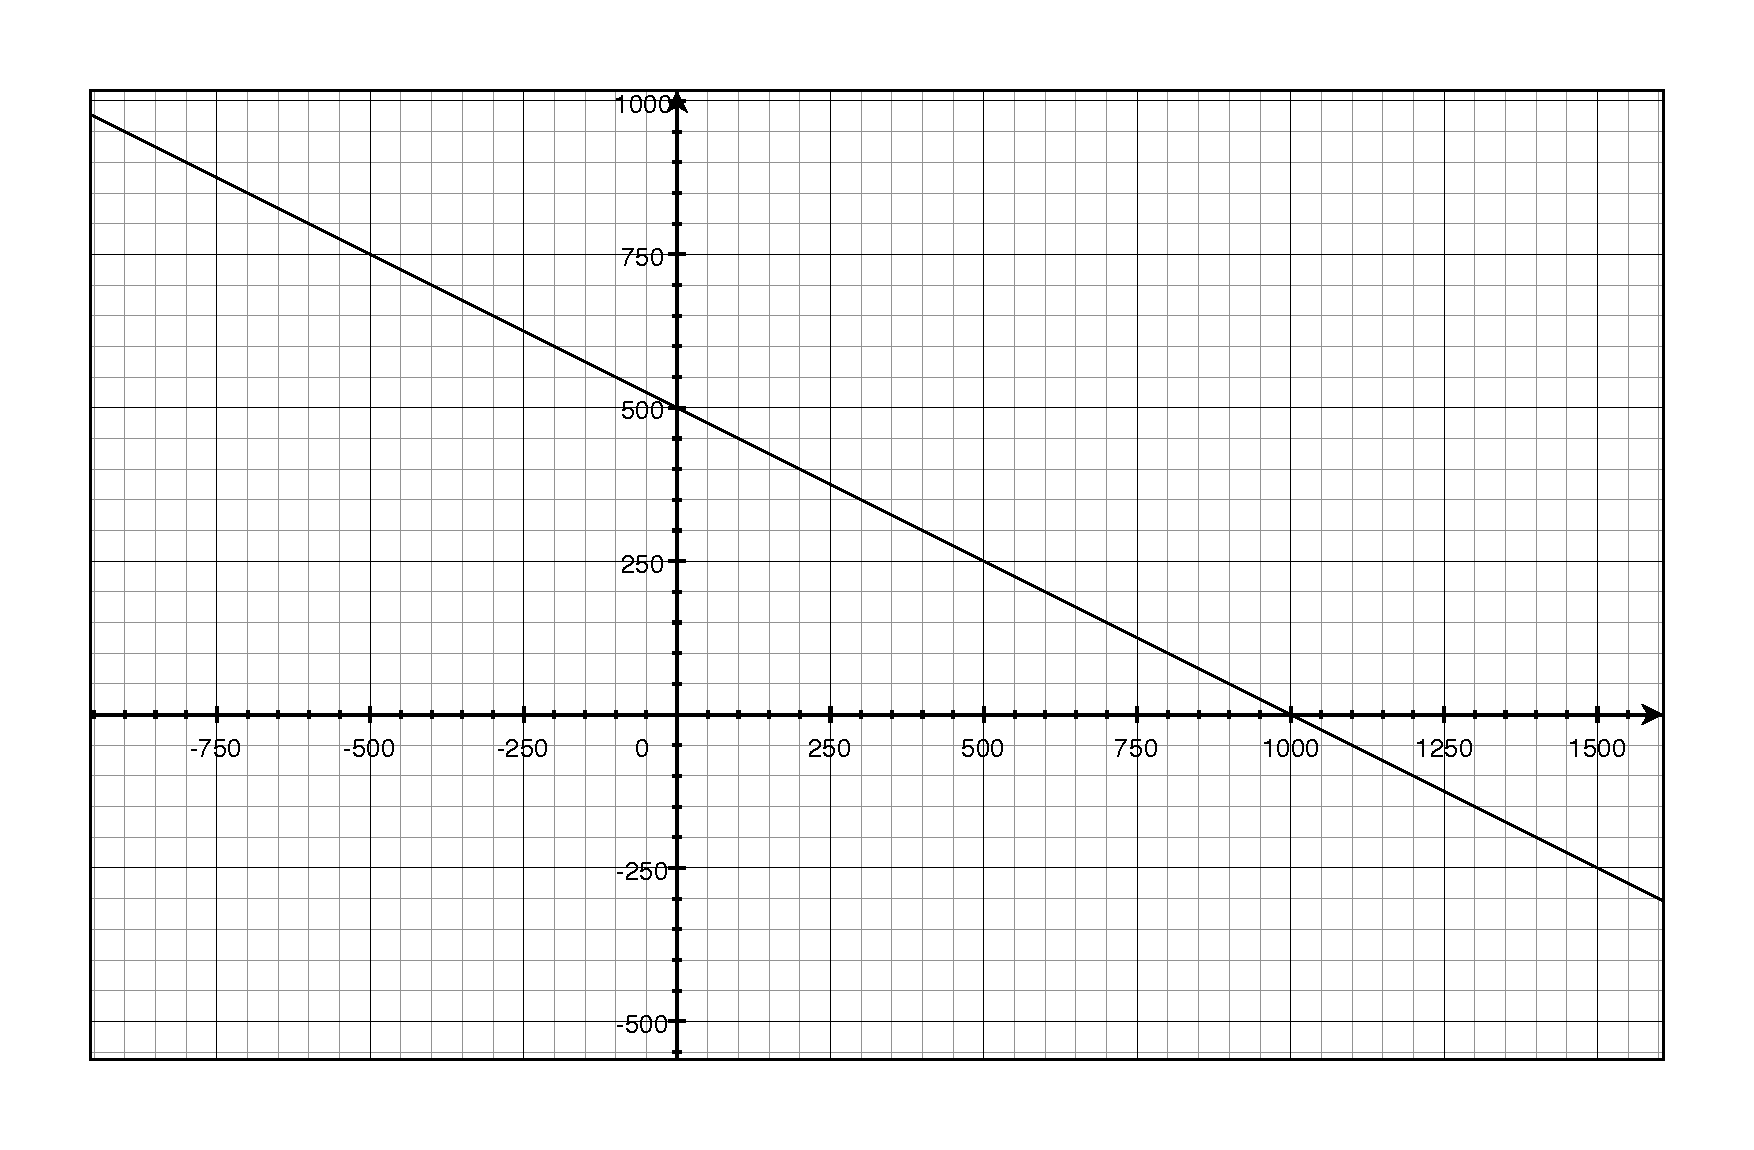
\includegraphics[width=7cm,height=5cm]{problem-21}
\end{figure}

The total weight is the number of fish times the average weight of each fish, or:

\[
  total(n) = n(500 - 0.5n)
\]

The total for 1,000 fish is: 
\[
  total(1000) = 1000(500 - 0.5(1000)) = 0
\]

When there are 1,000 fish, there isn't enough food to go around and the fish are so malnourished that they have an
average weight of 0.

\end{itemize}

\section{Pages 65-66}
\begin{itemize}

\item[1]
$y = x^2 + 1$ is the graph of $y=x^2$ shifted up 1.

\begin{figure}[H]
  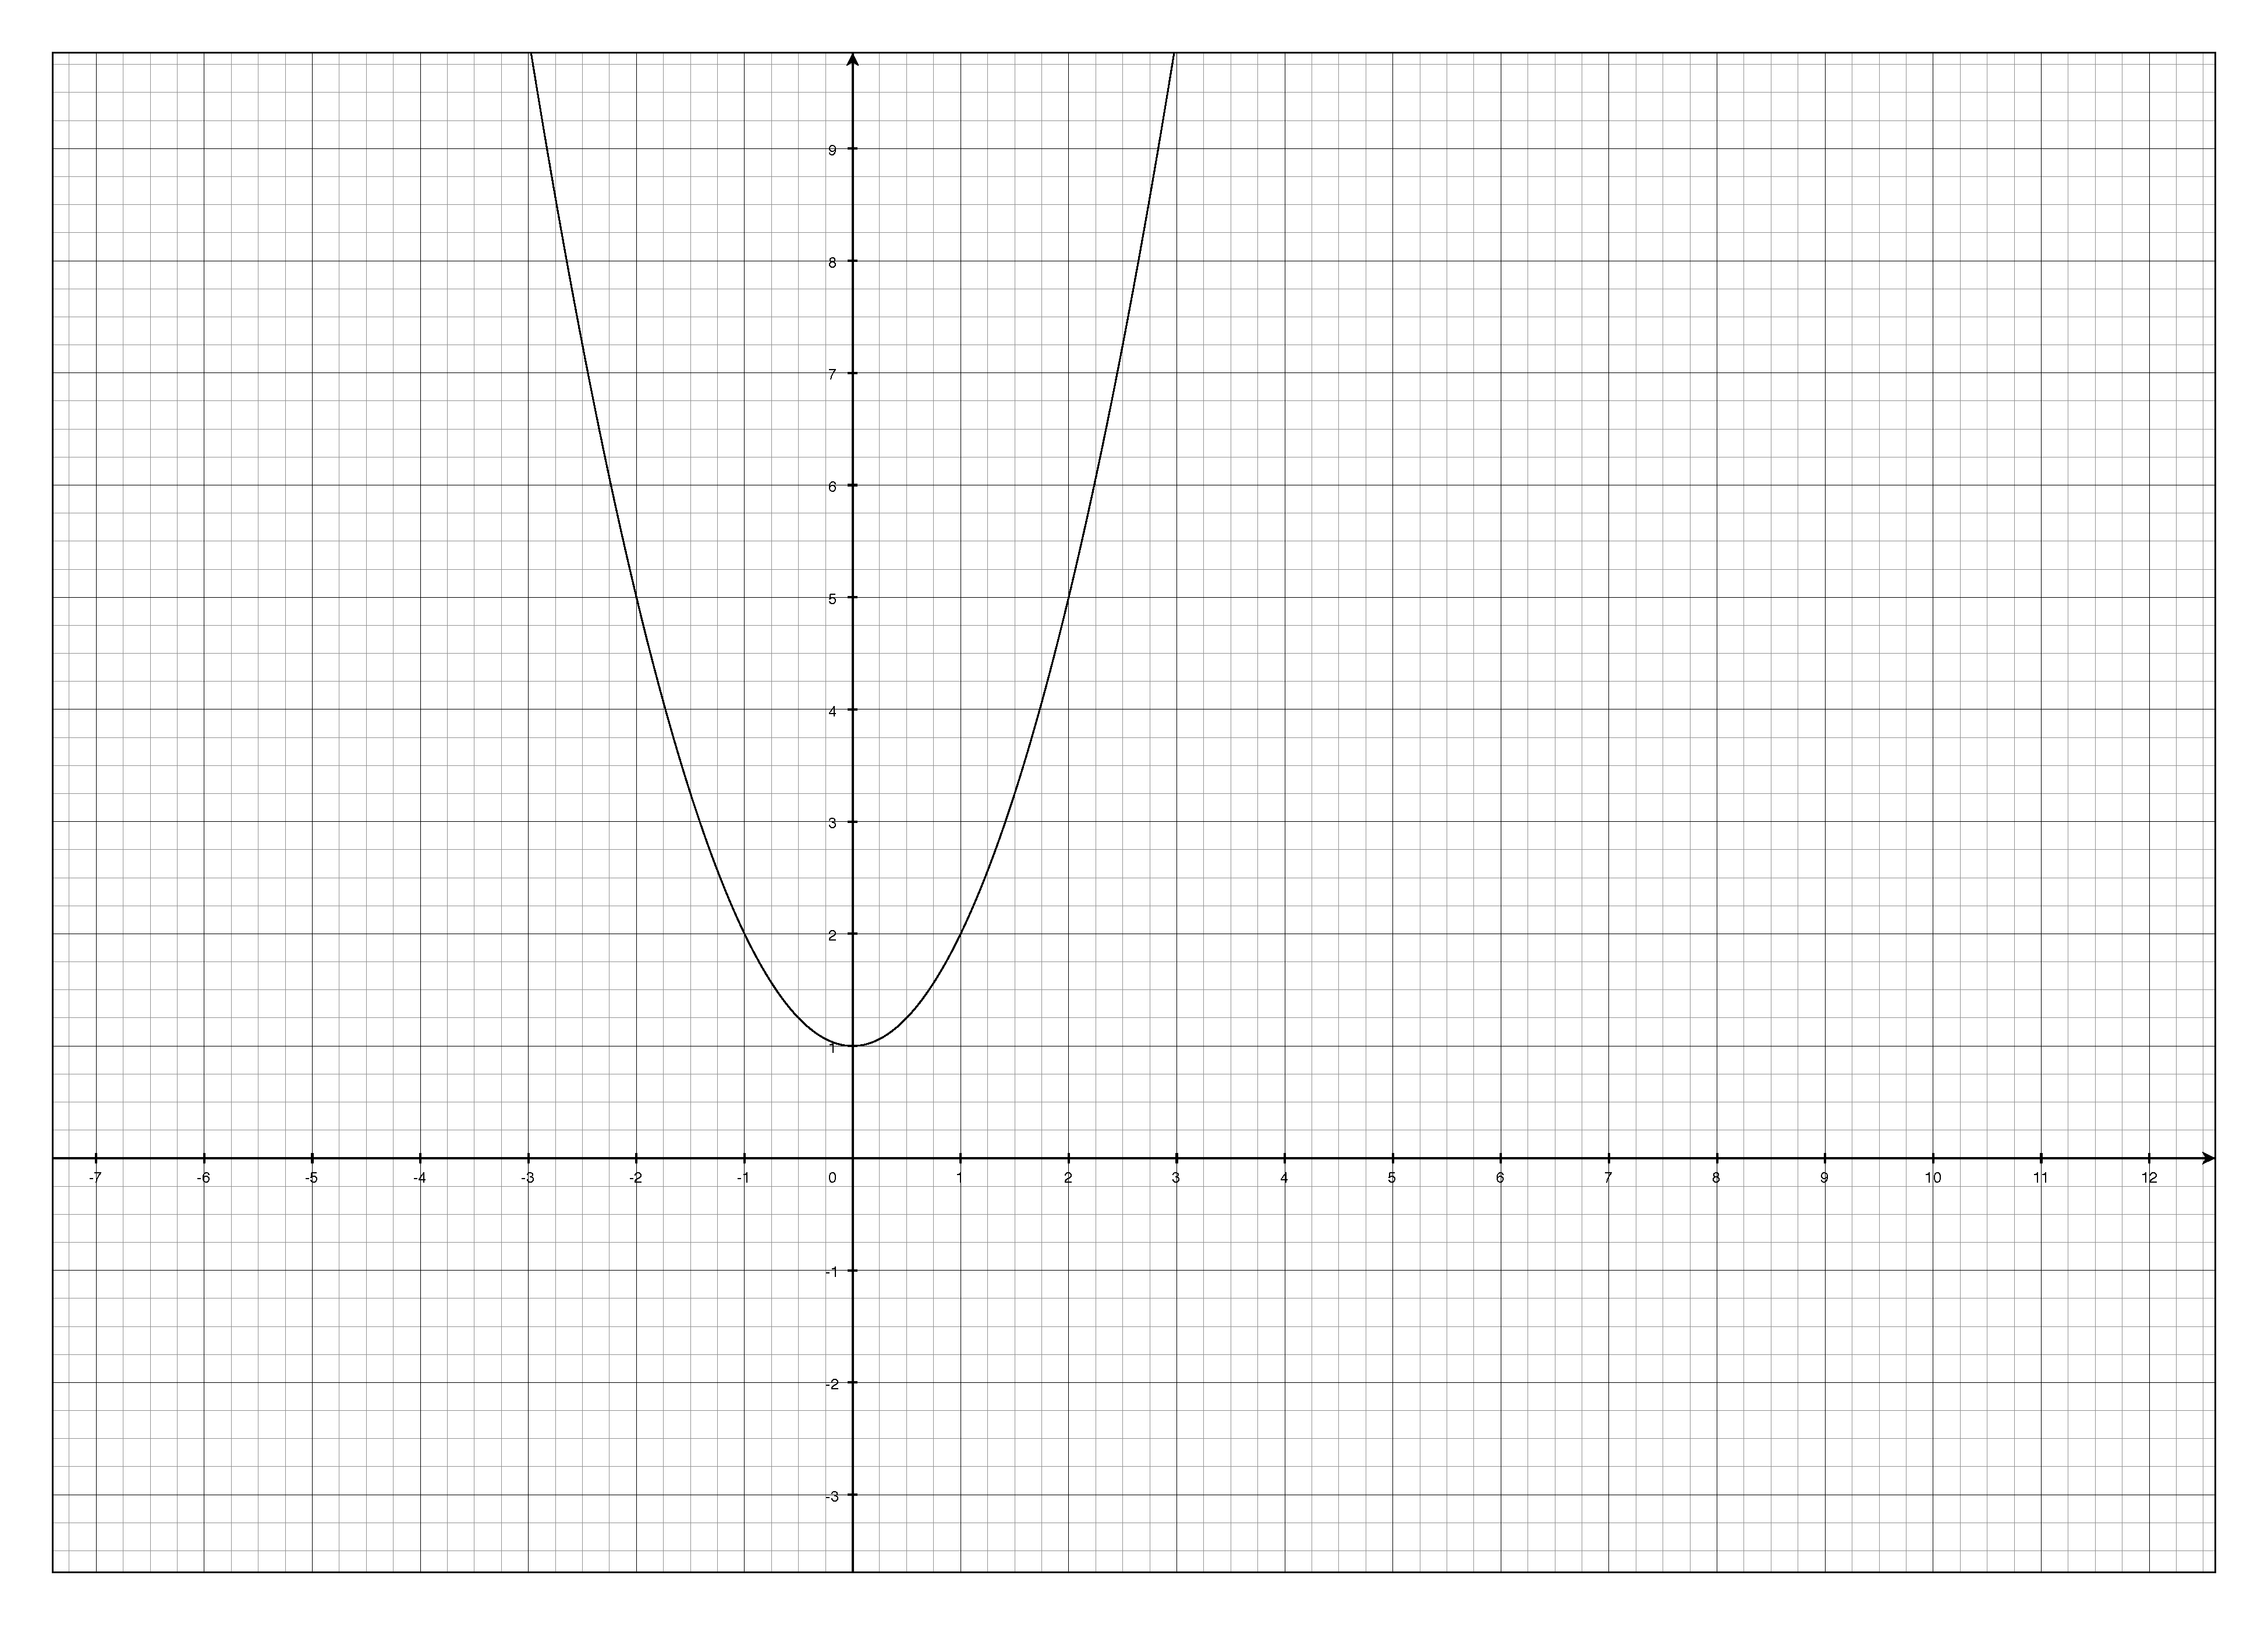
\includegraphics[width=7cm,height=5cm]{1.8-1.eps}
\end{figure}

\item[3]
$y = (x - 3)^2$ is the graph of $y=x^2$ shifted right by 3.

\begin{figure}[H]
  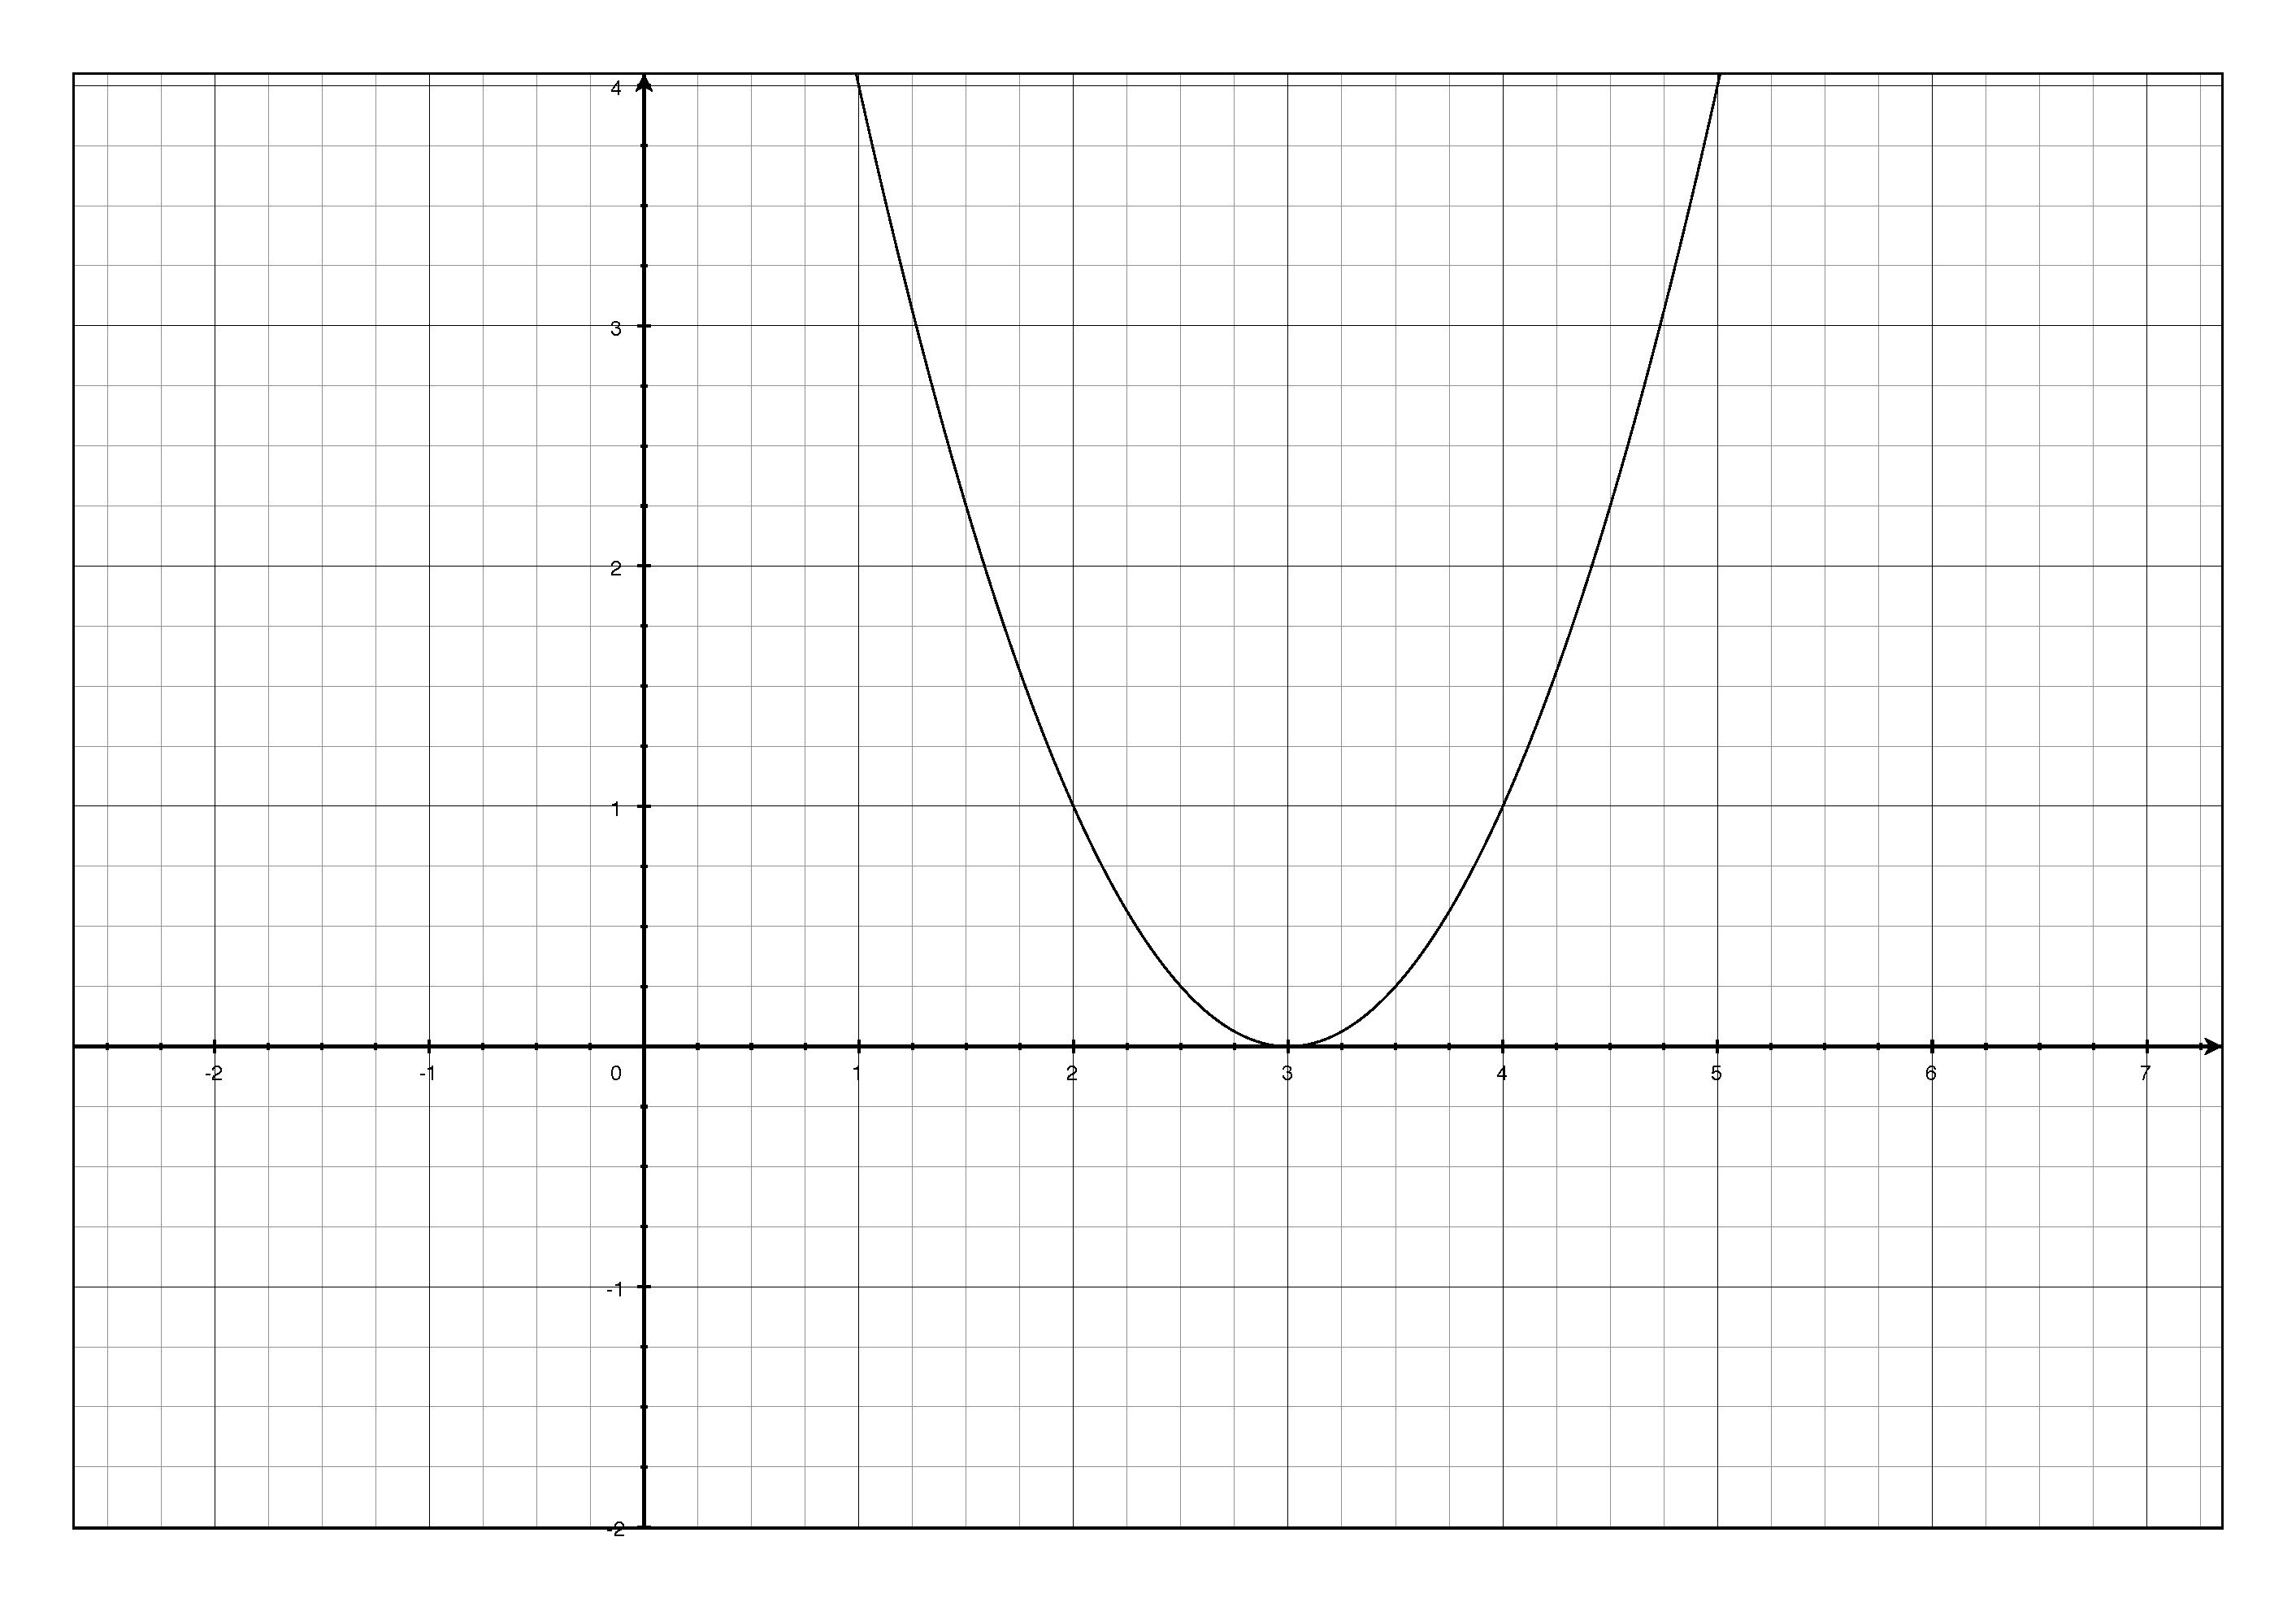
\includegraphics[width=7cm,height=5cm]{1.8-3.eps}
\end{figure}

\item[5]
\begin{align*}
  y &= x^2 - 4x + 4 \\
   &= (x - 2)^2 \\
\end{align*}

So the graph is $y=x^2$ shifted right by 2.

\begin{figure}[H]
  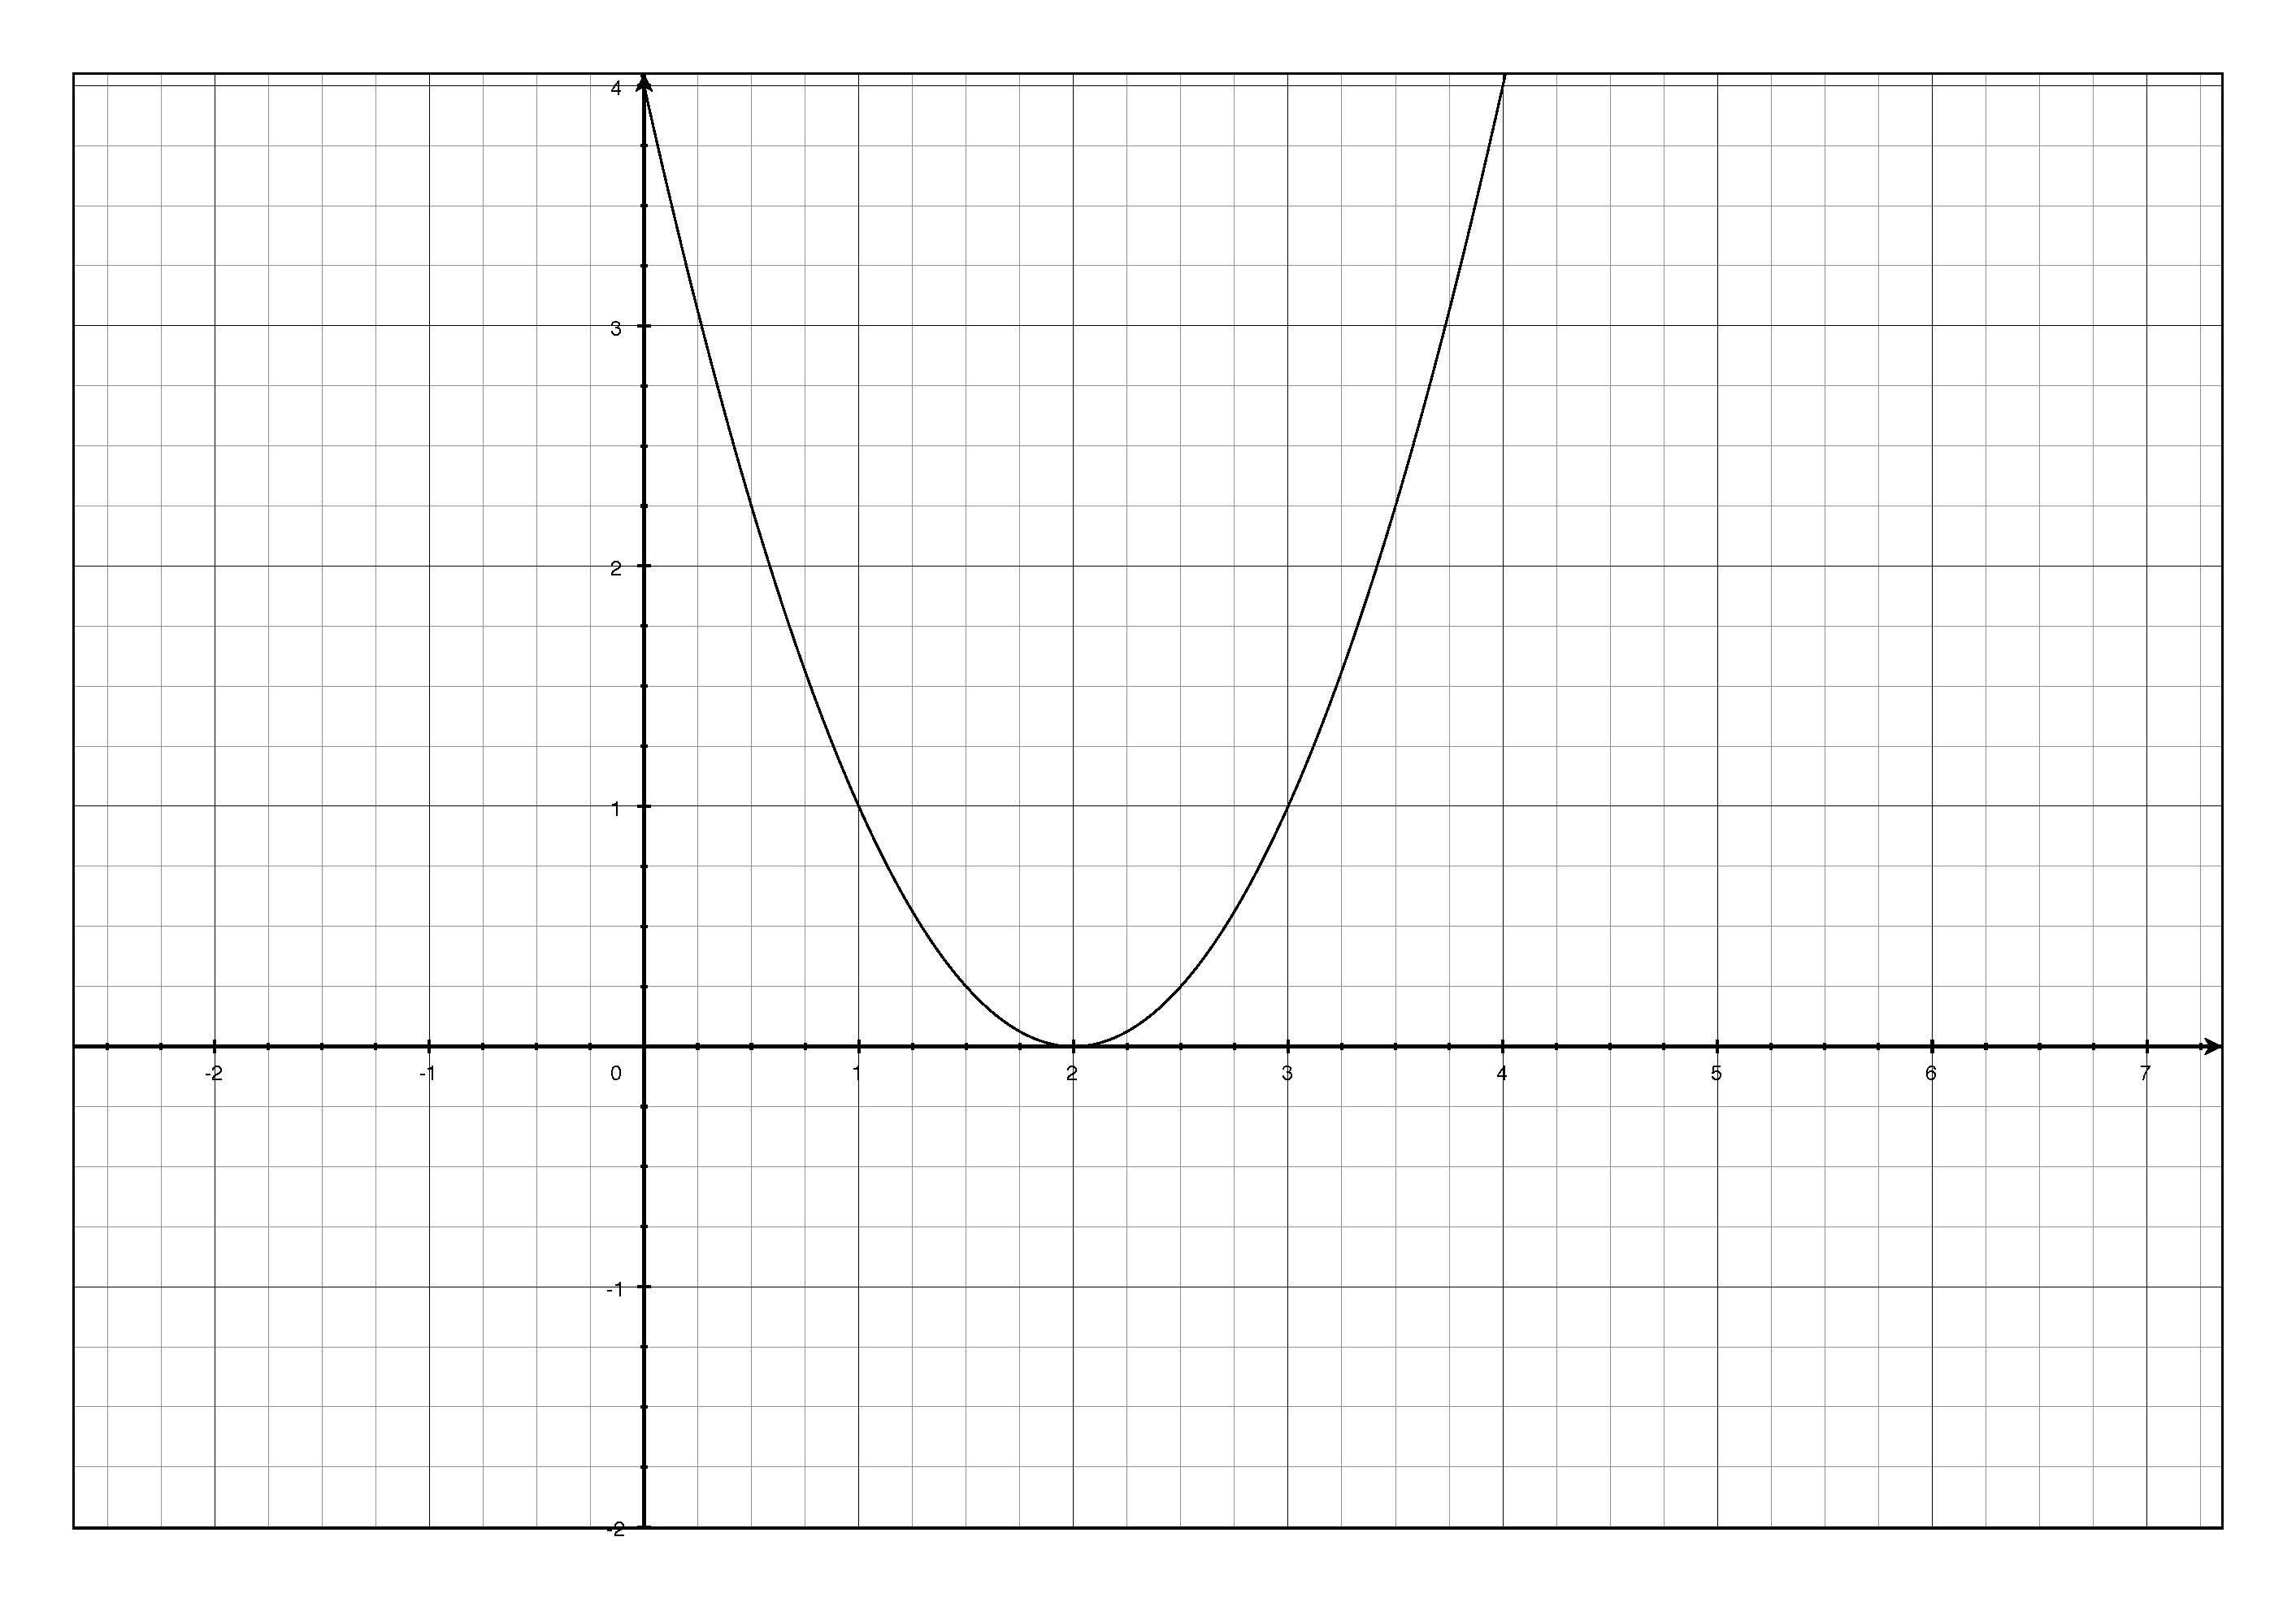
\includegraphics[width=7cm,height=5cm]{1.8-5.eps}
\end{figure}

\item[6]
\begin{align*}
  y &= x^2 - 4x + 3 \\
    &= x^2 - 4x + 4 - 4 + 3 \\
    &= (x - 2)^2 - 1 \\
\end{align*}

So the graph is $y=x^2$ shifted right 2 and down 1.

\begin{figure}[H]
  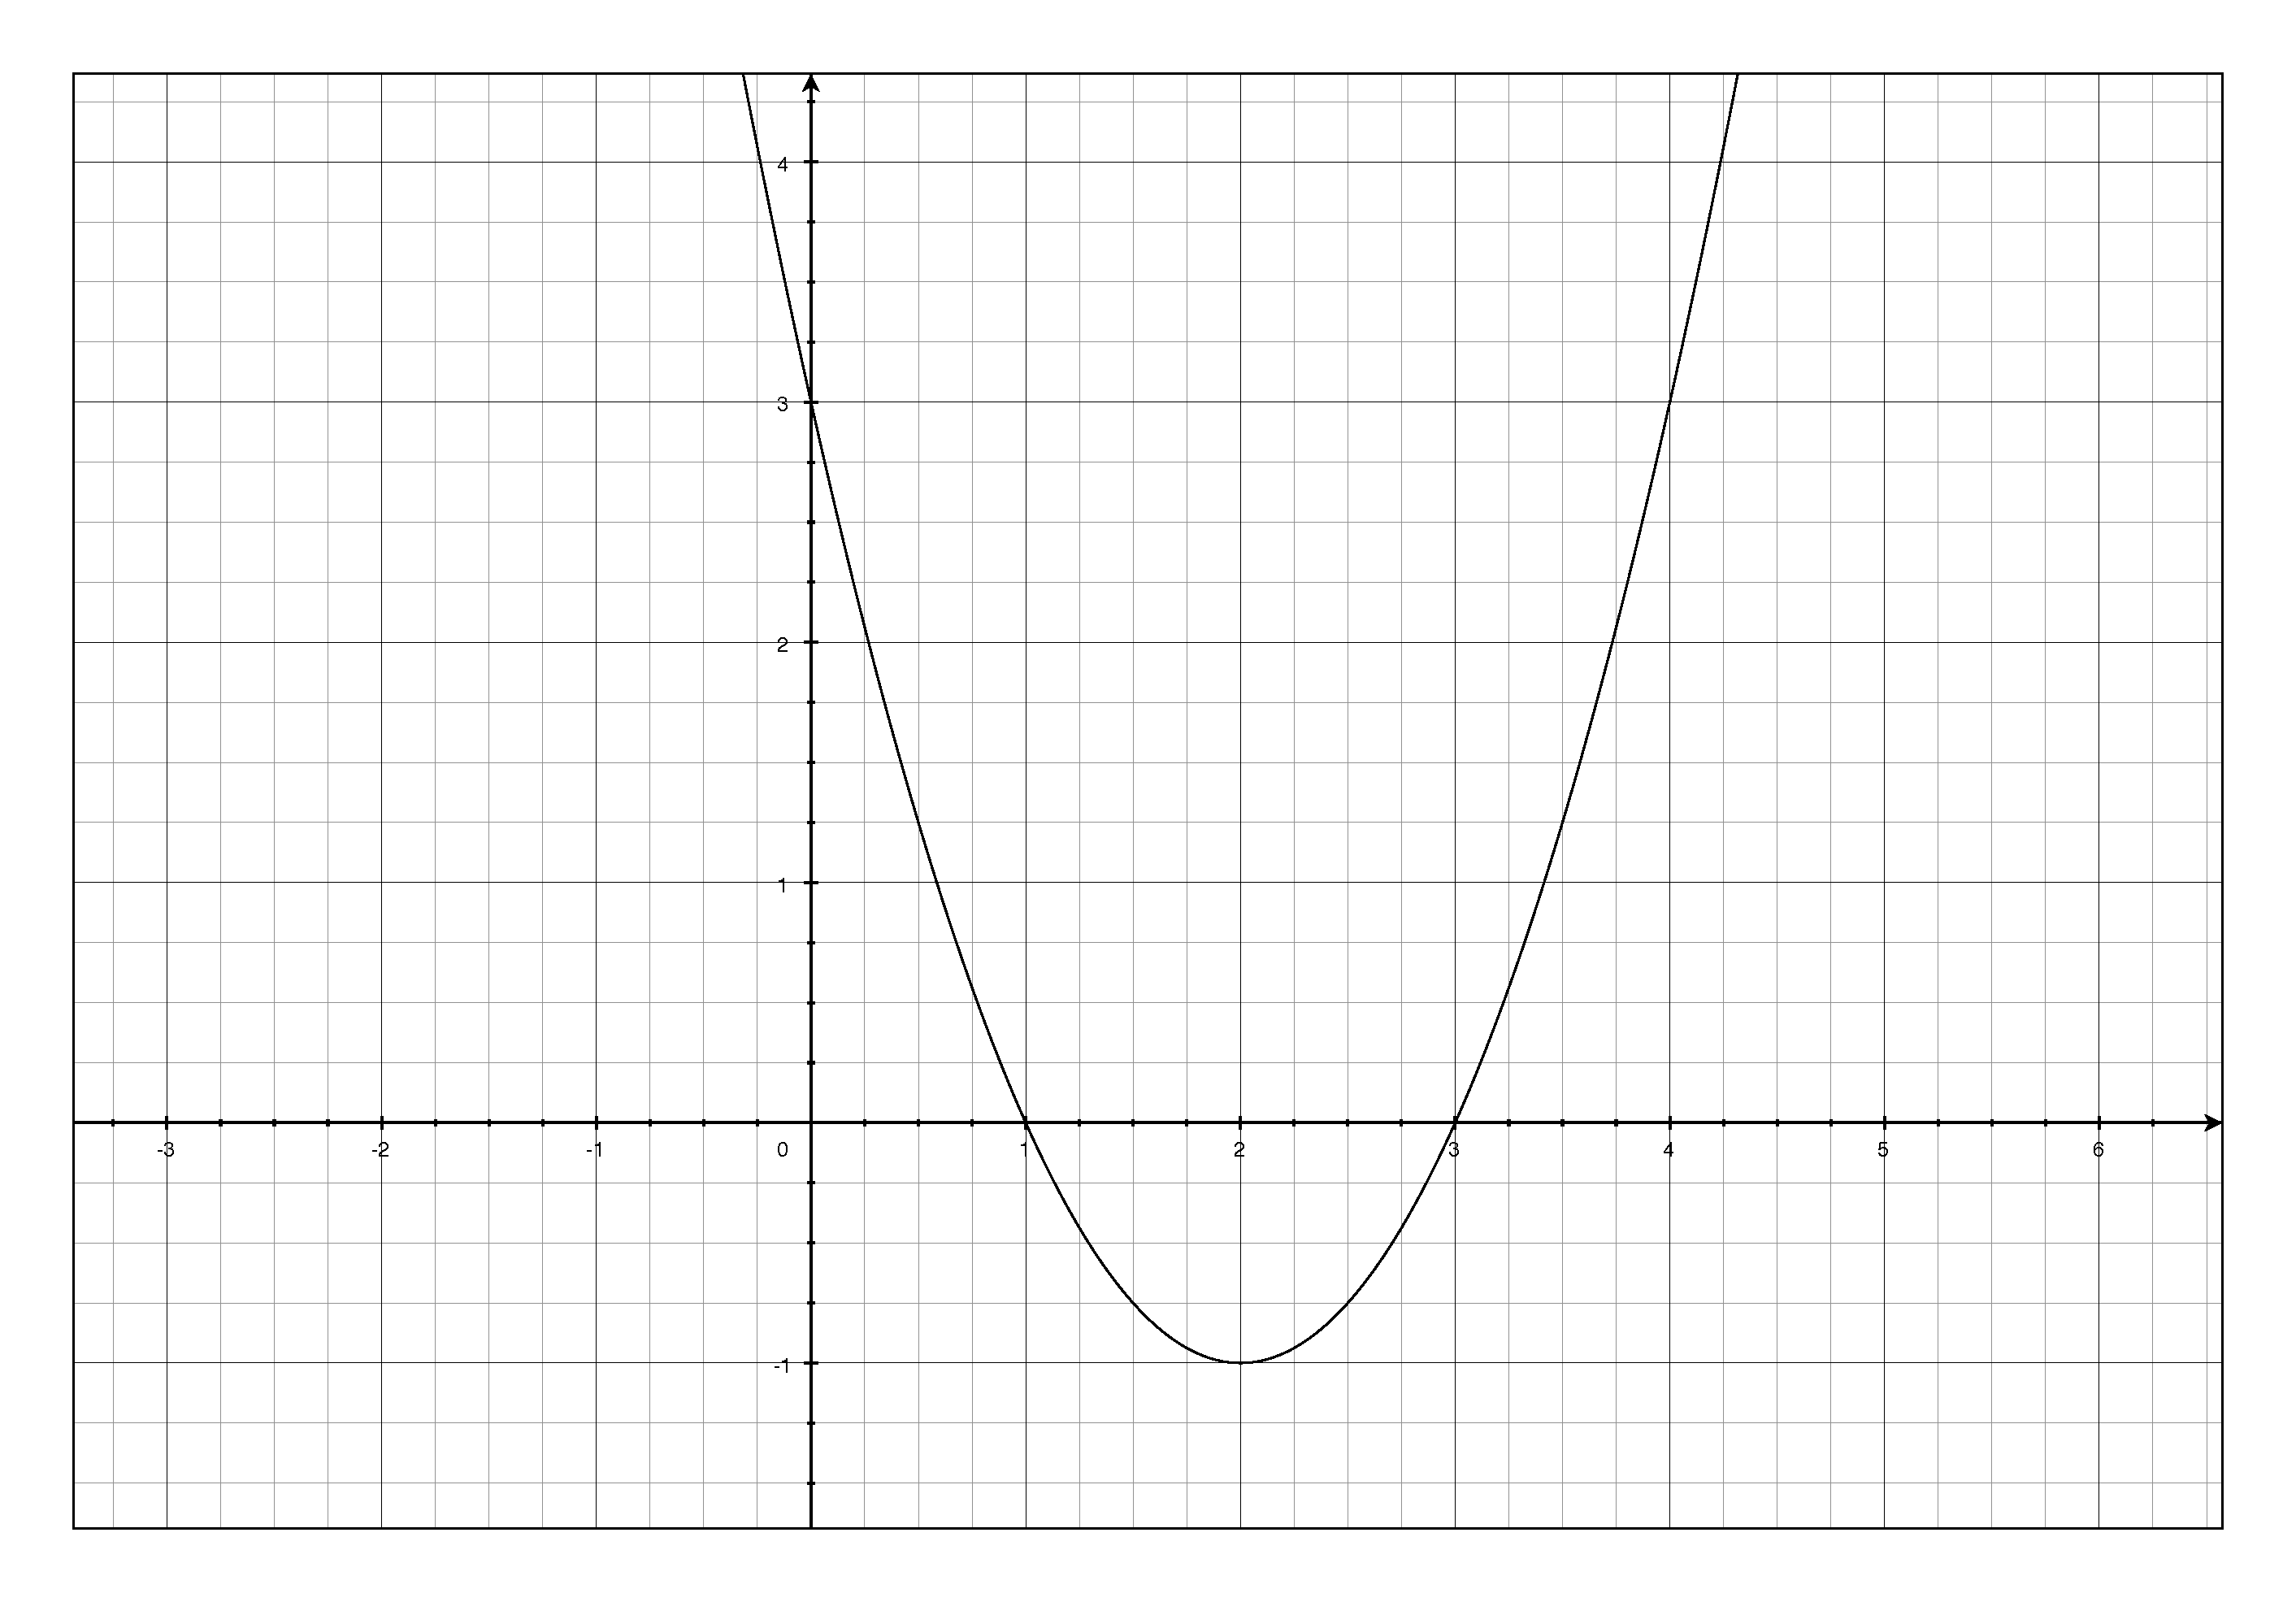
\includegraphics[width=7cm,height=5cm]{1.8-6.eps}
\end{figure}

\item[19]
See the back of the book.
% \begin{itemize}

% \item[a]
% \begin{figure}[H]
%   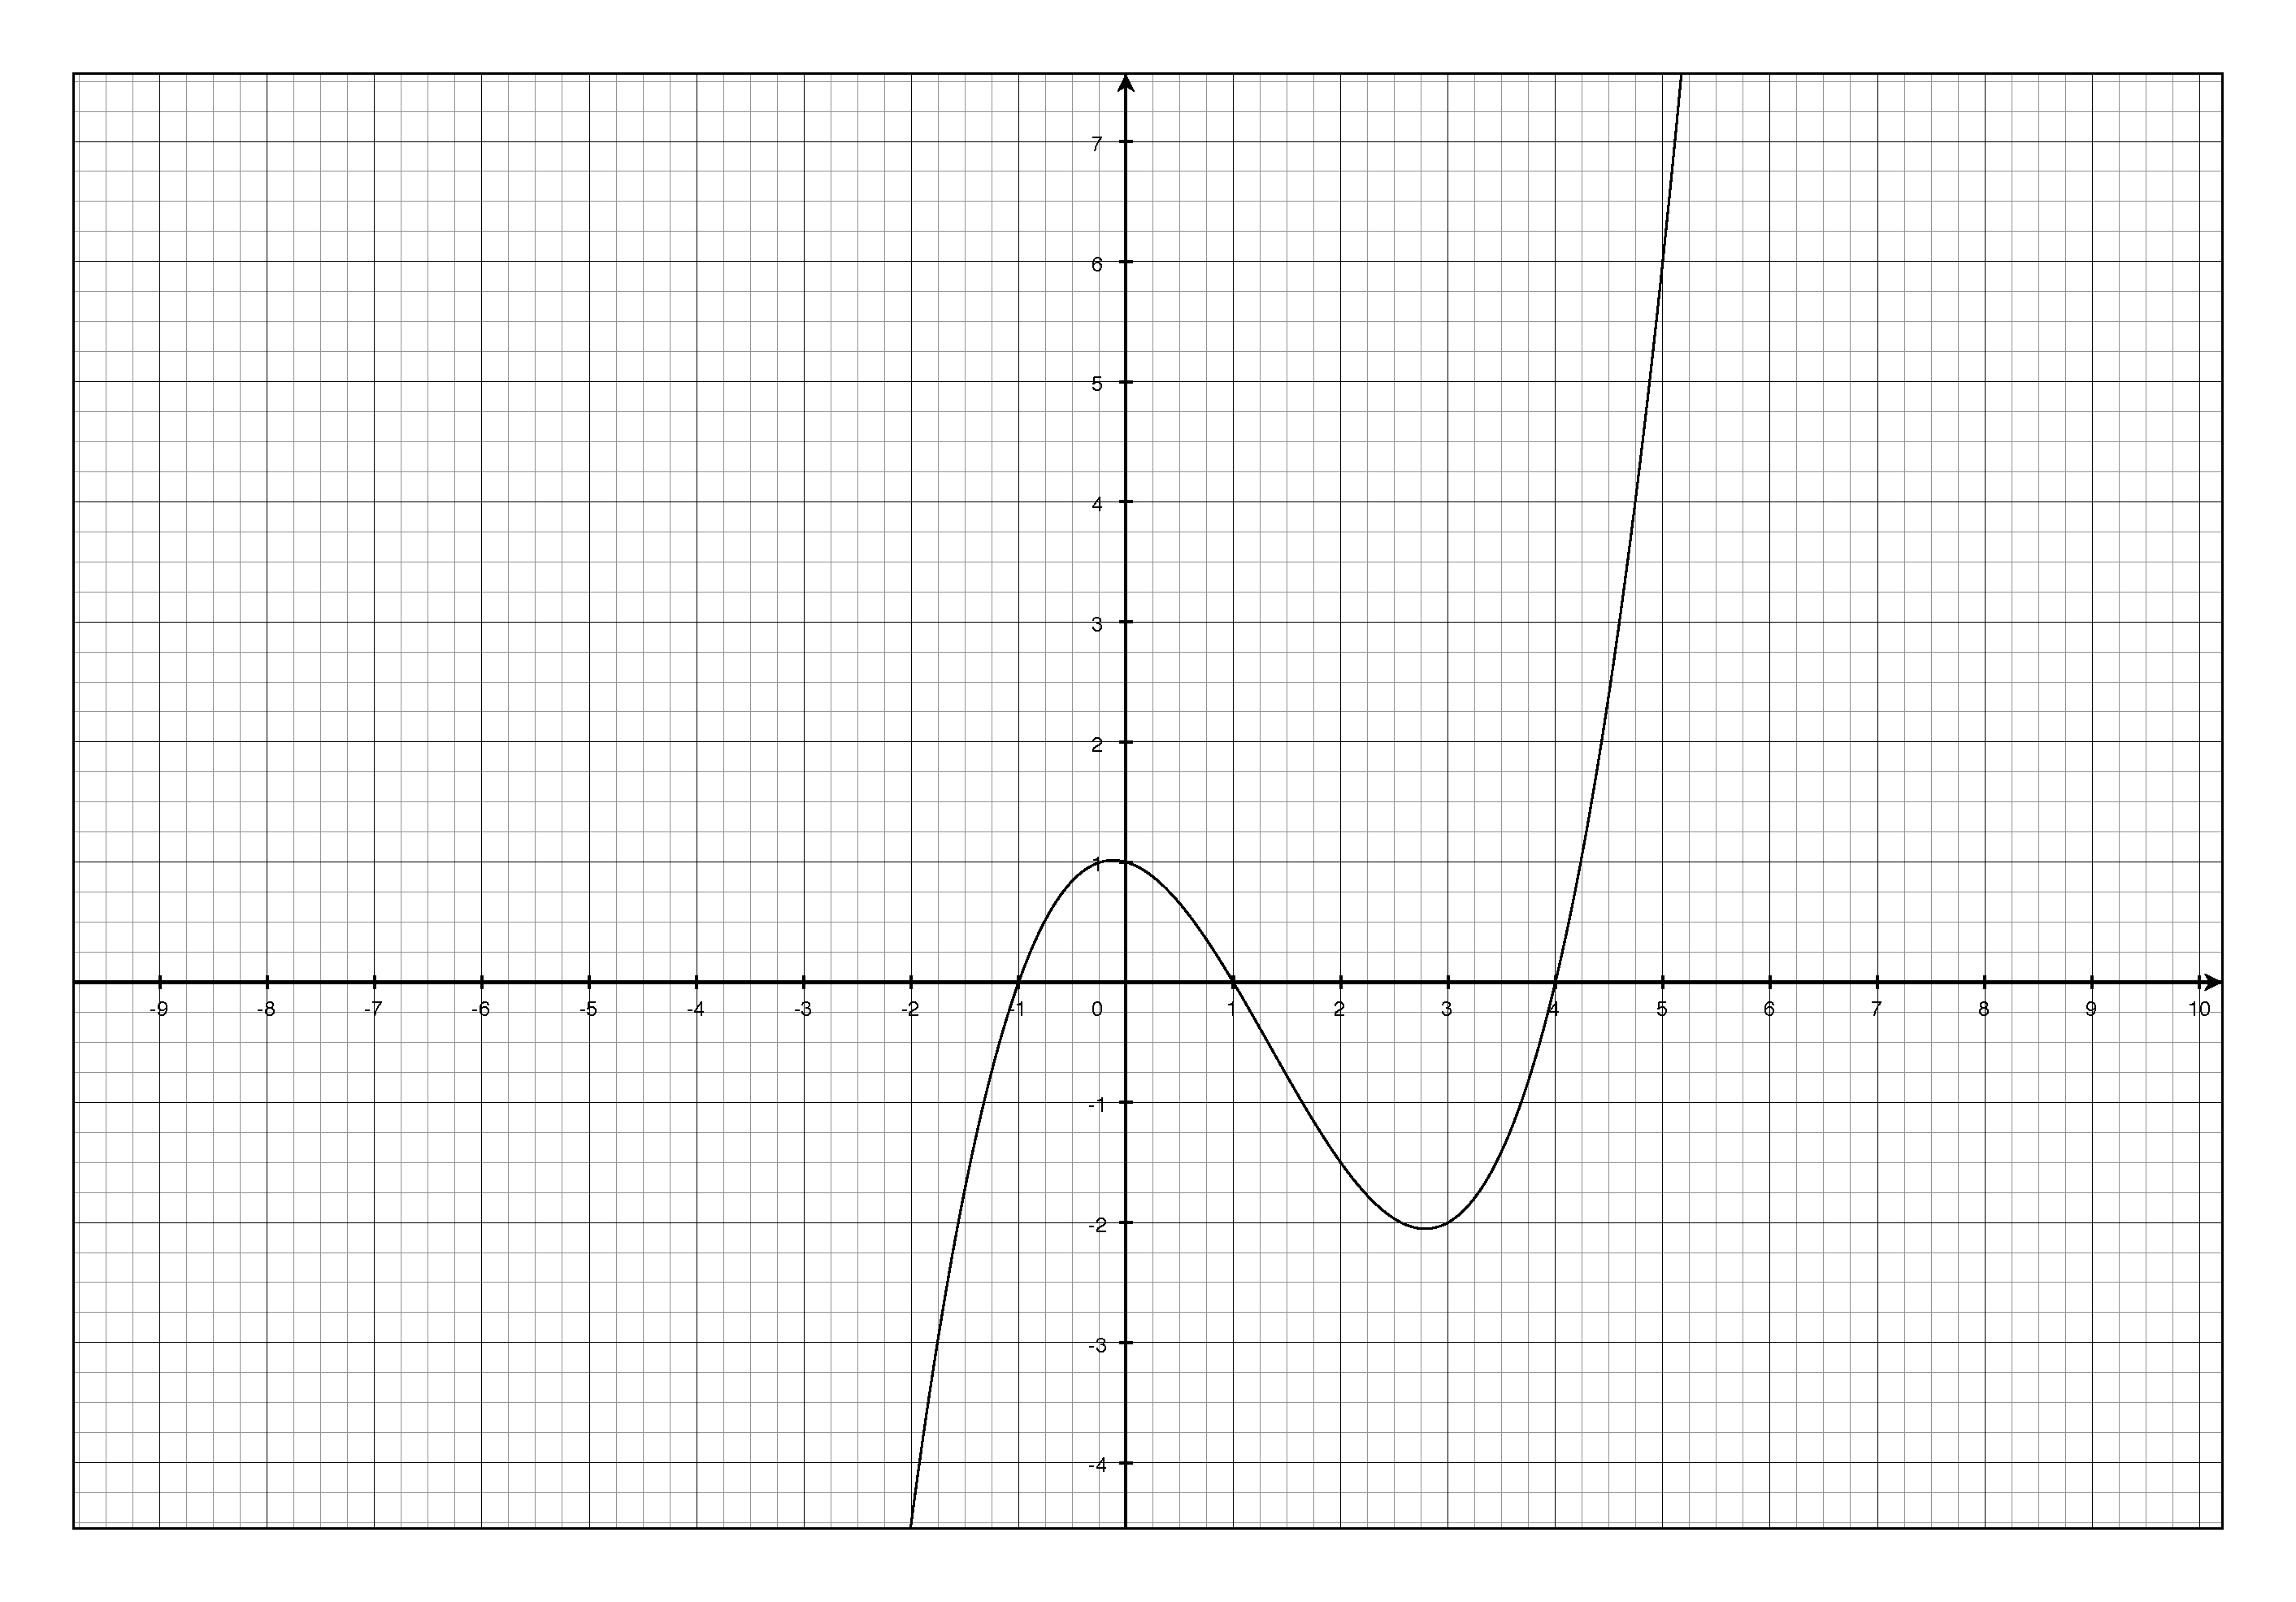
\includegraphics[width=7cm,height=5cm]{1.8-19-a.eps}
%   \caption{$y = f(x-1)$}
% \end{figure}

% \item[b]
% \begin{figure}[H]
%   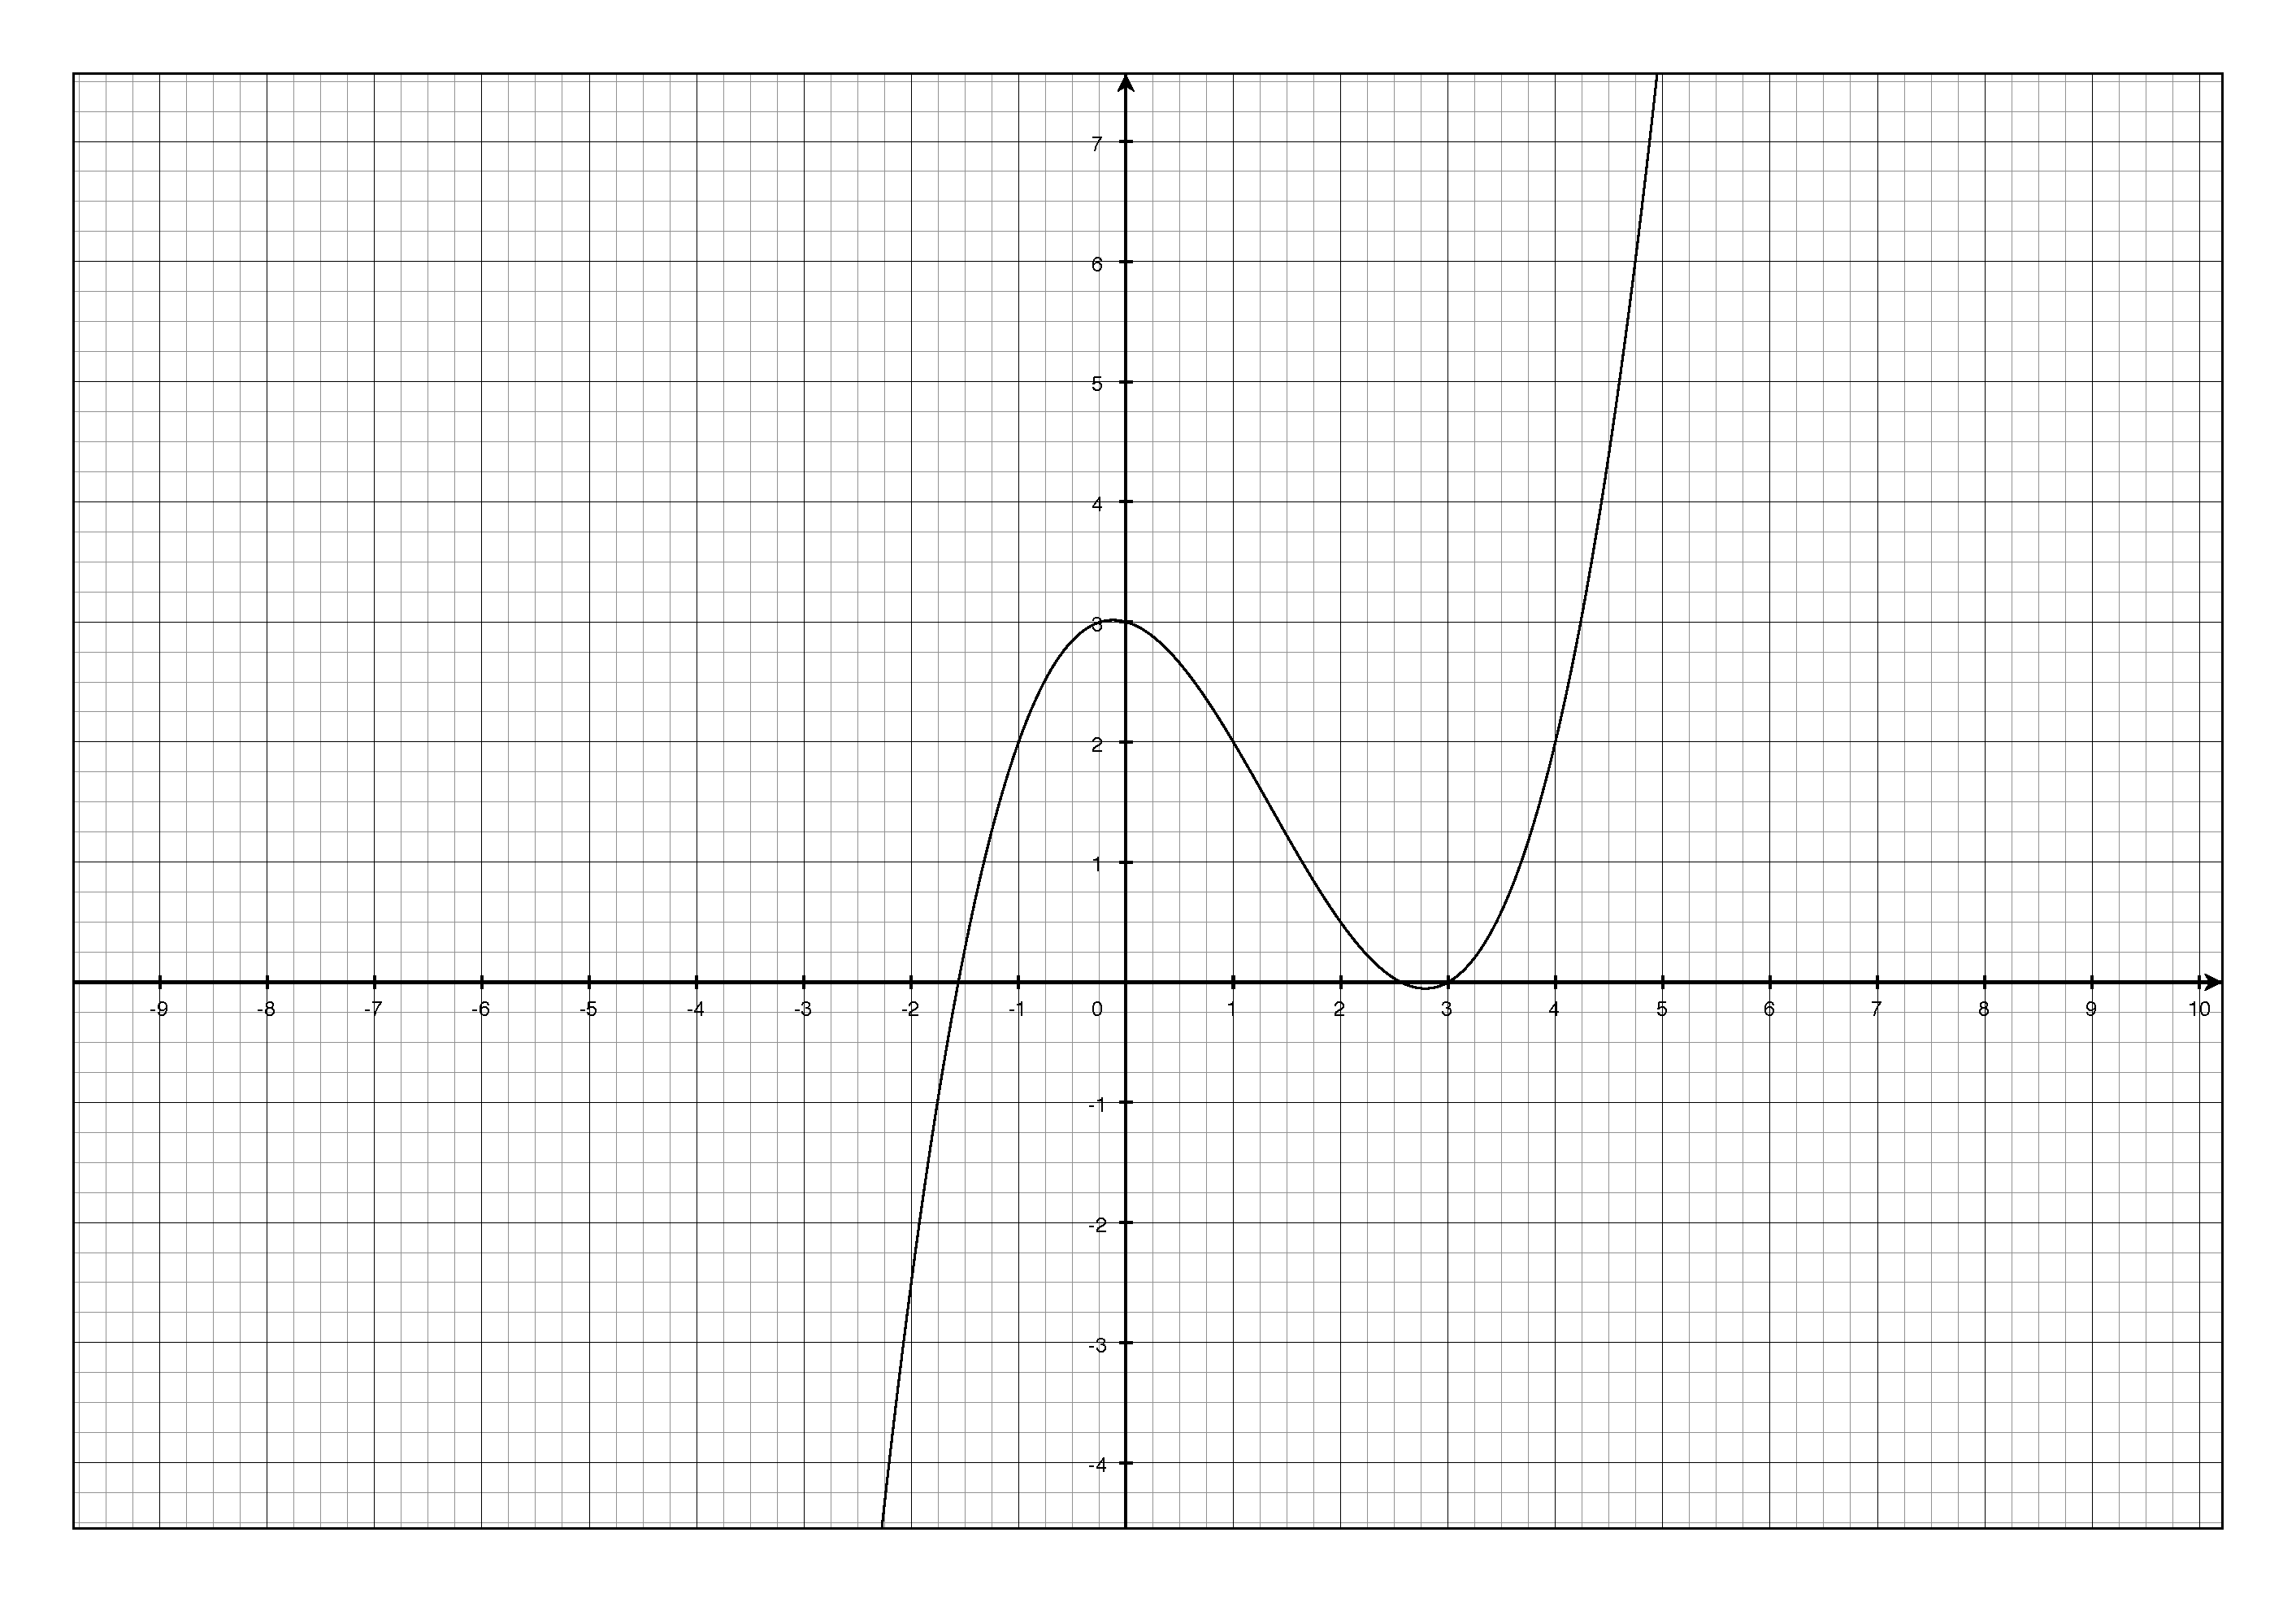
\includegraphics[width=7cm,height=5cm]{1.8-19-b.eps}
%   \caption{$y = f(x-1) + 2$}
% \end{figure}

% \item[c]
% \begin{figure}[H]
%   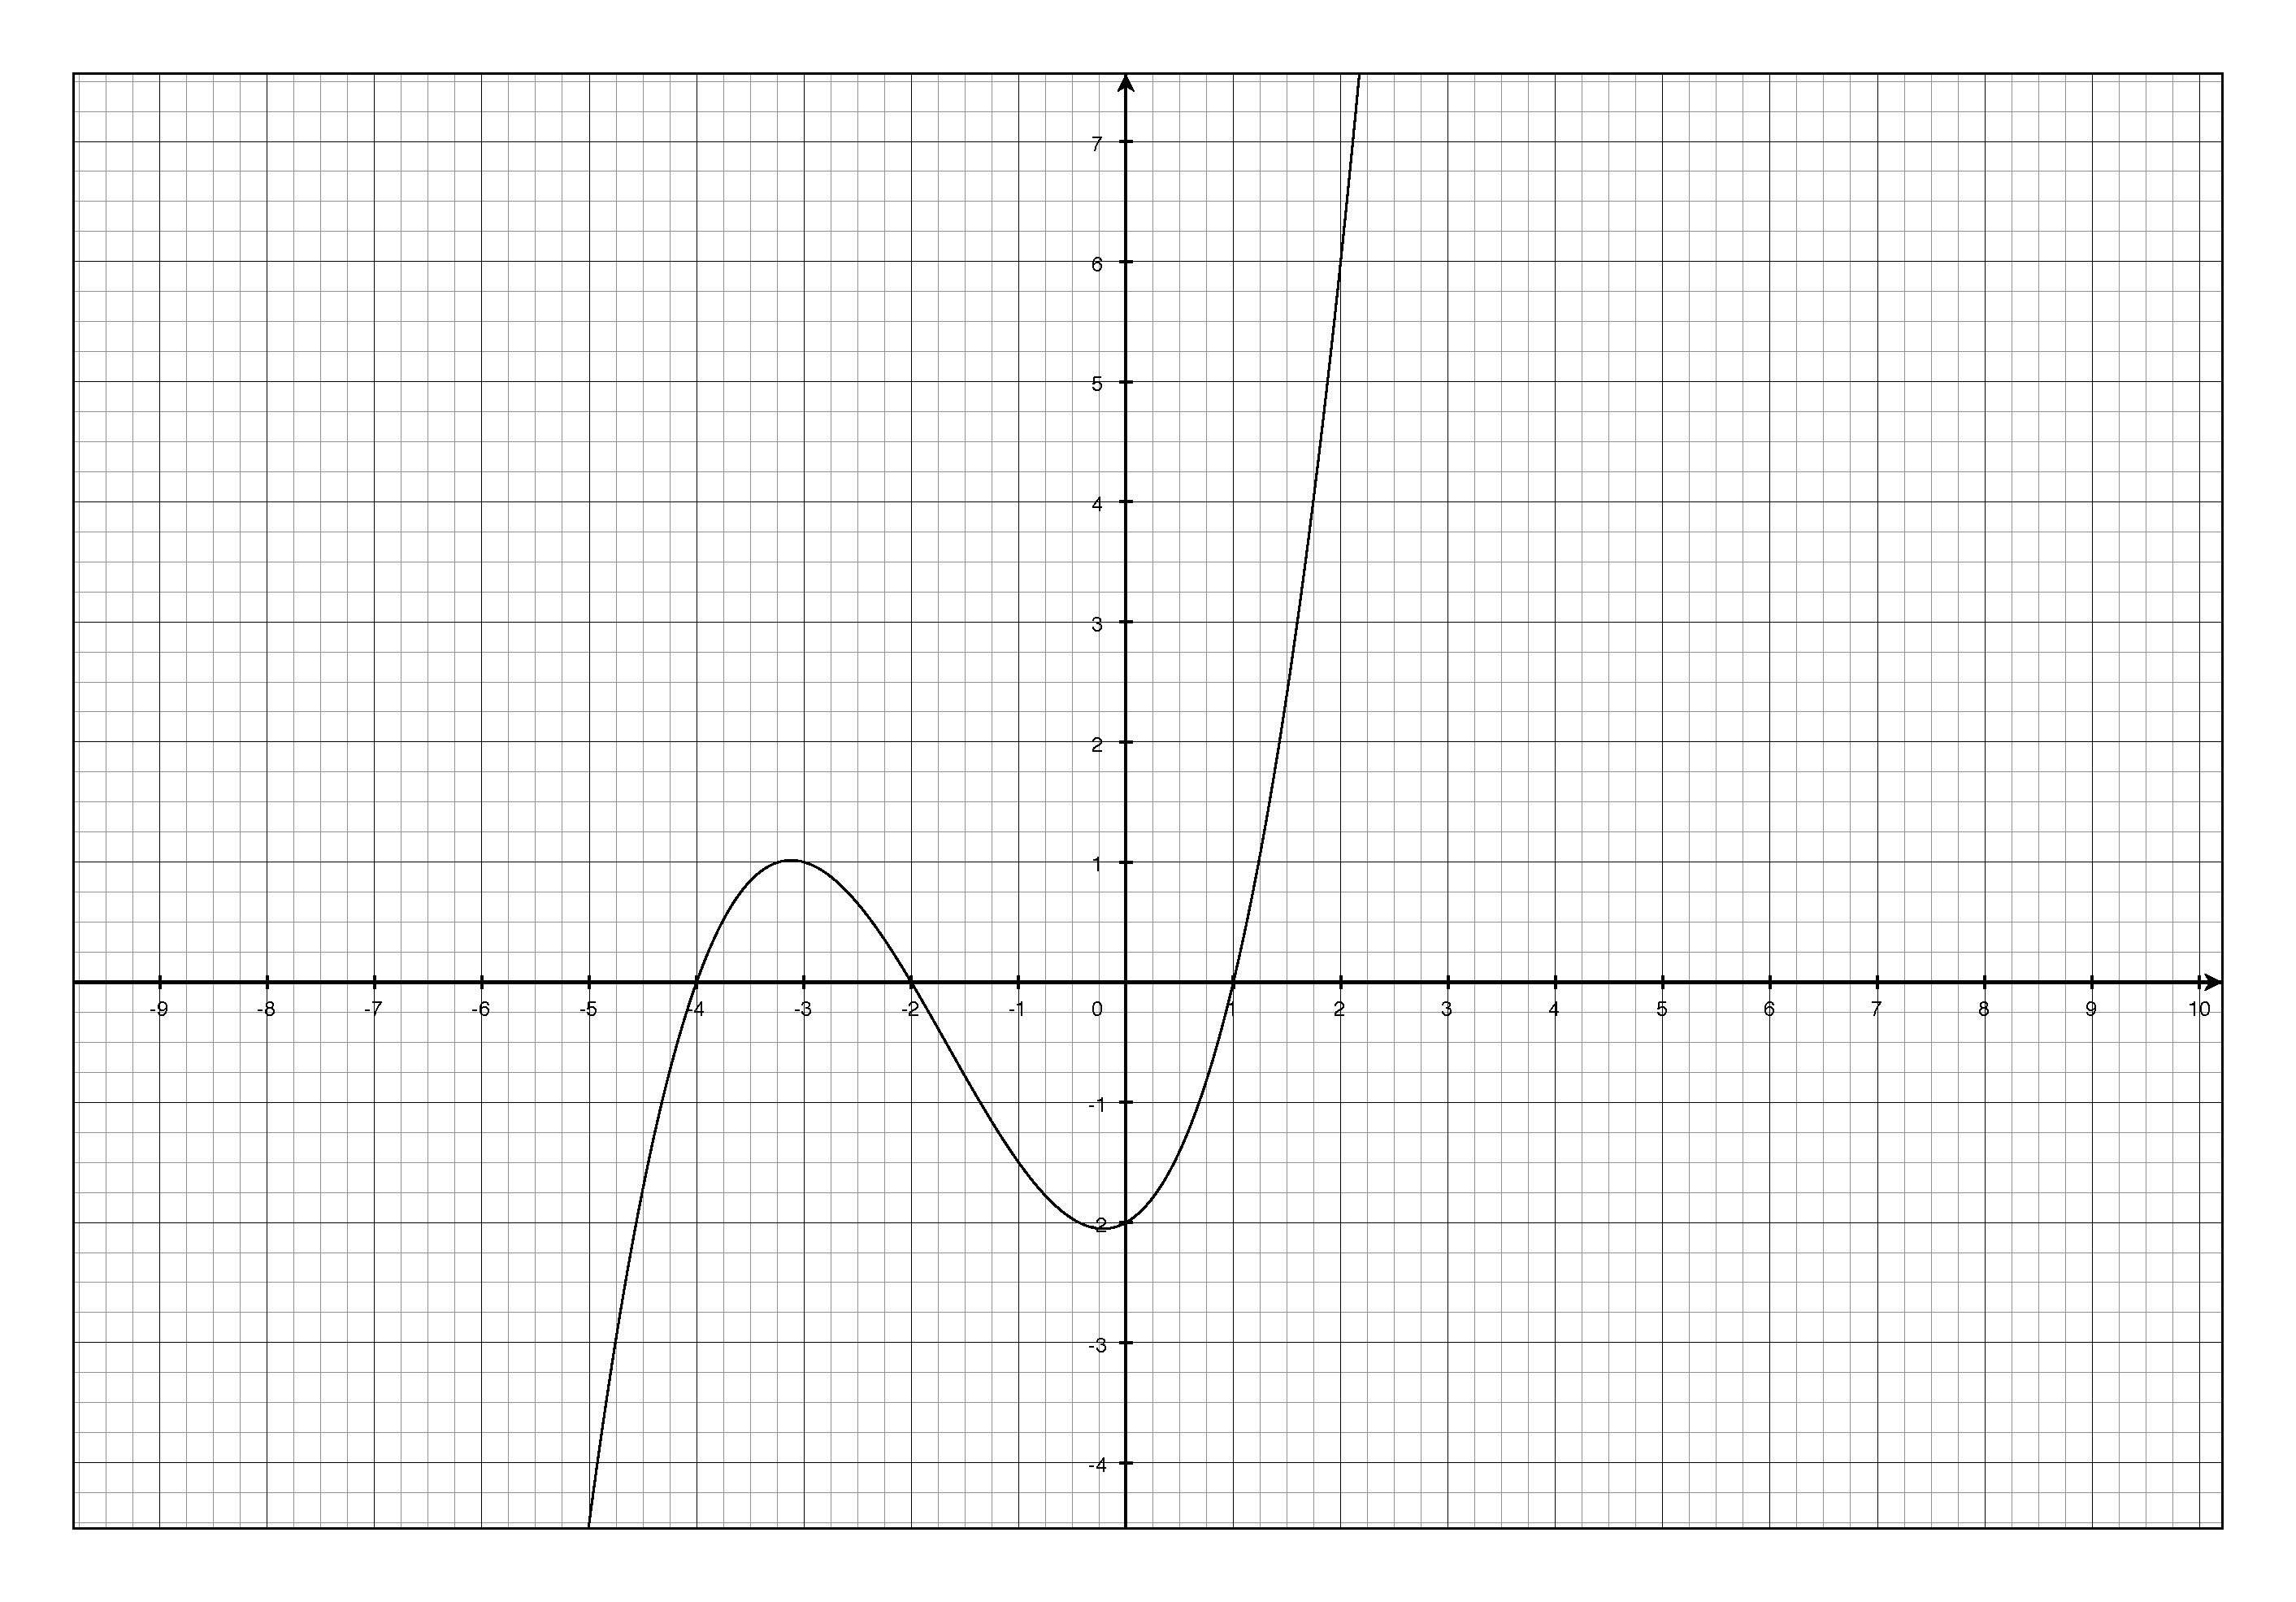
\includegraphics[width=7cm,height=5cm]{1.8-19-c.eps}
%   \caption{$y = f(x+2)$}
% \end{figure}

% \item[d]
% \begin{figure}[H]
%   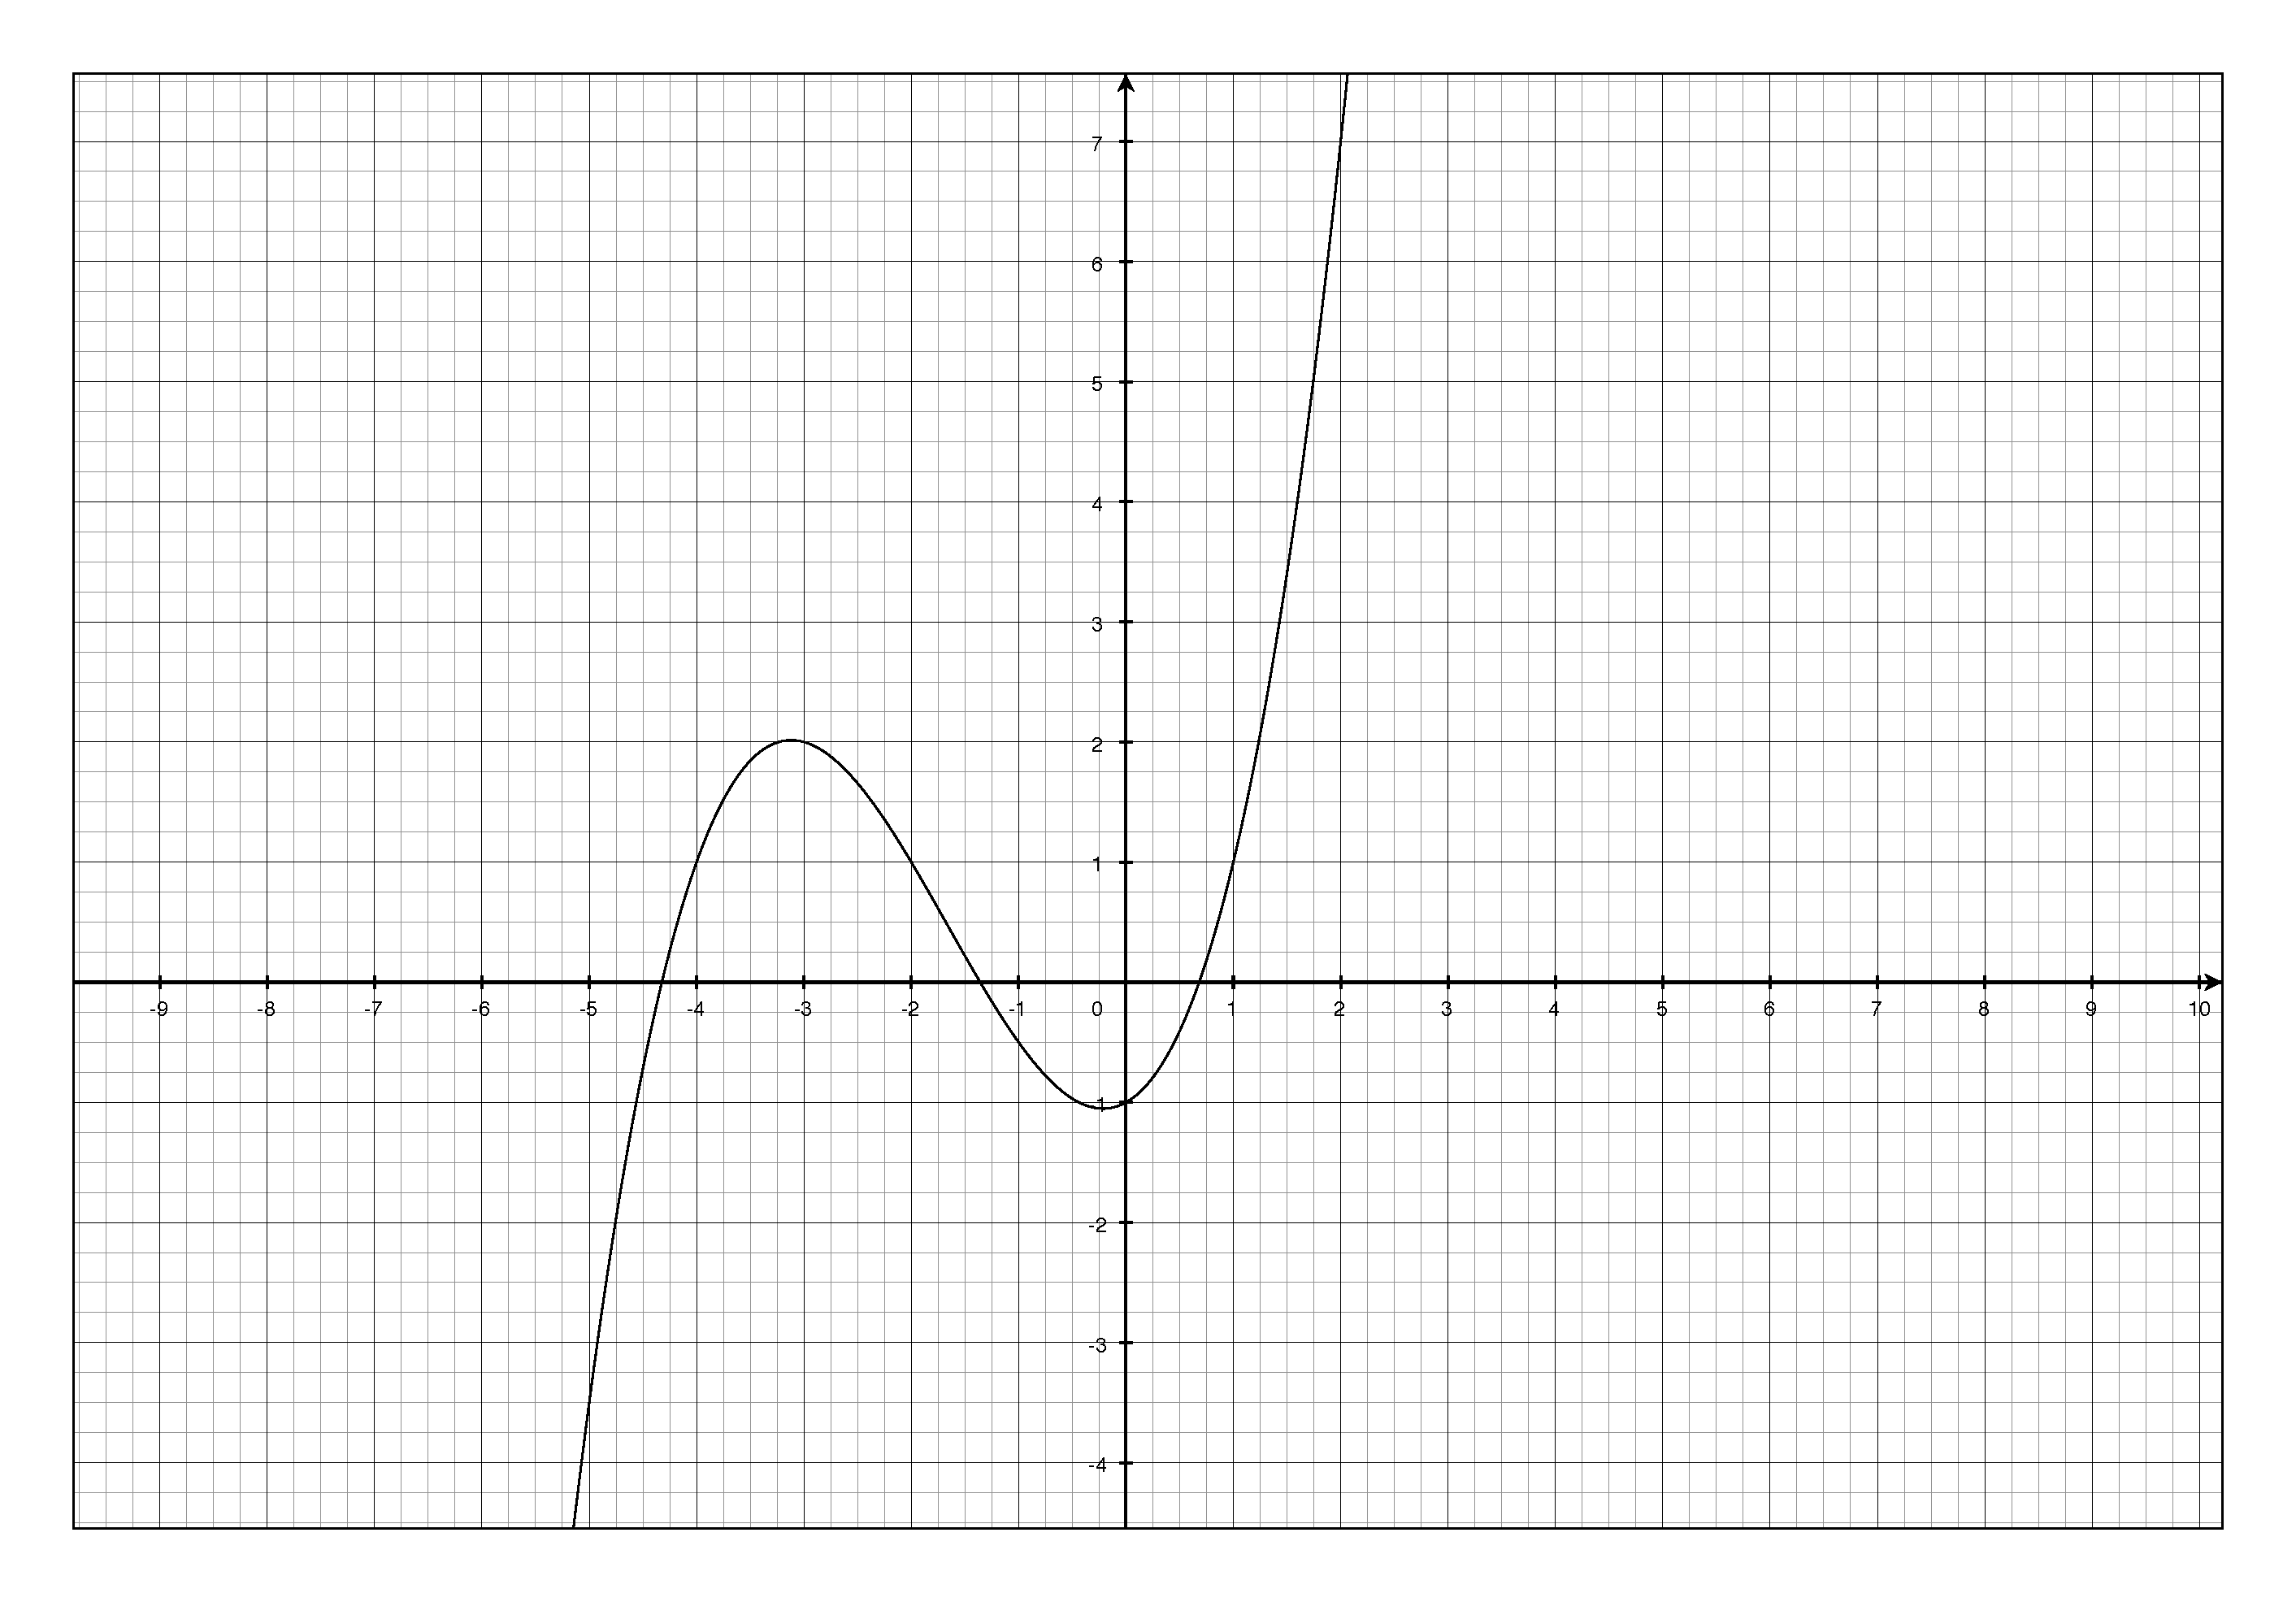
\includegraphics[width=7cm,height=5cm]{1.8-19-d.eps}
%   \caption{$y = f(x+2) + 1$}
% \end{figure}

% \item[e]
% \begin{figure}[H]
%   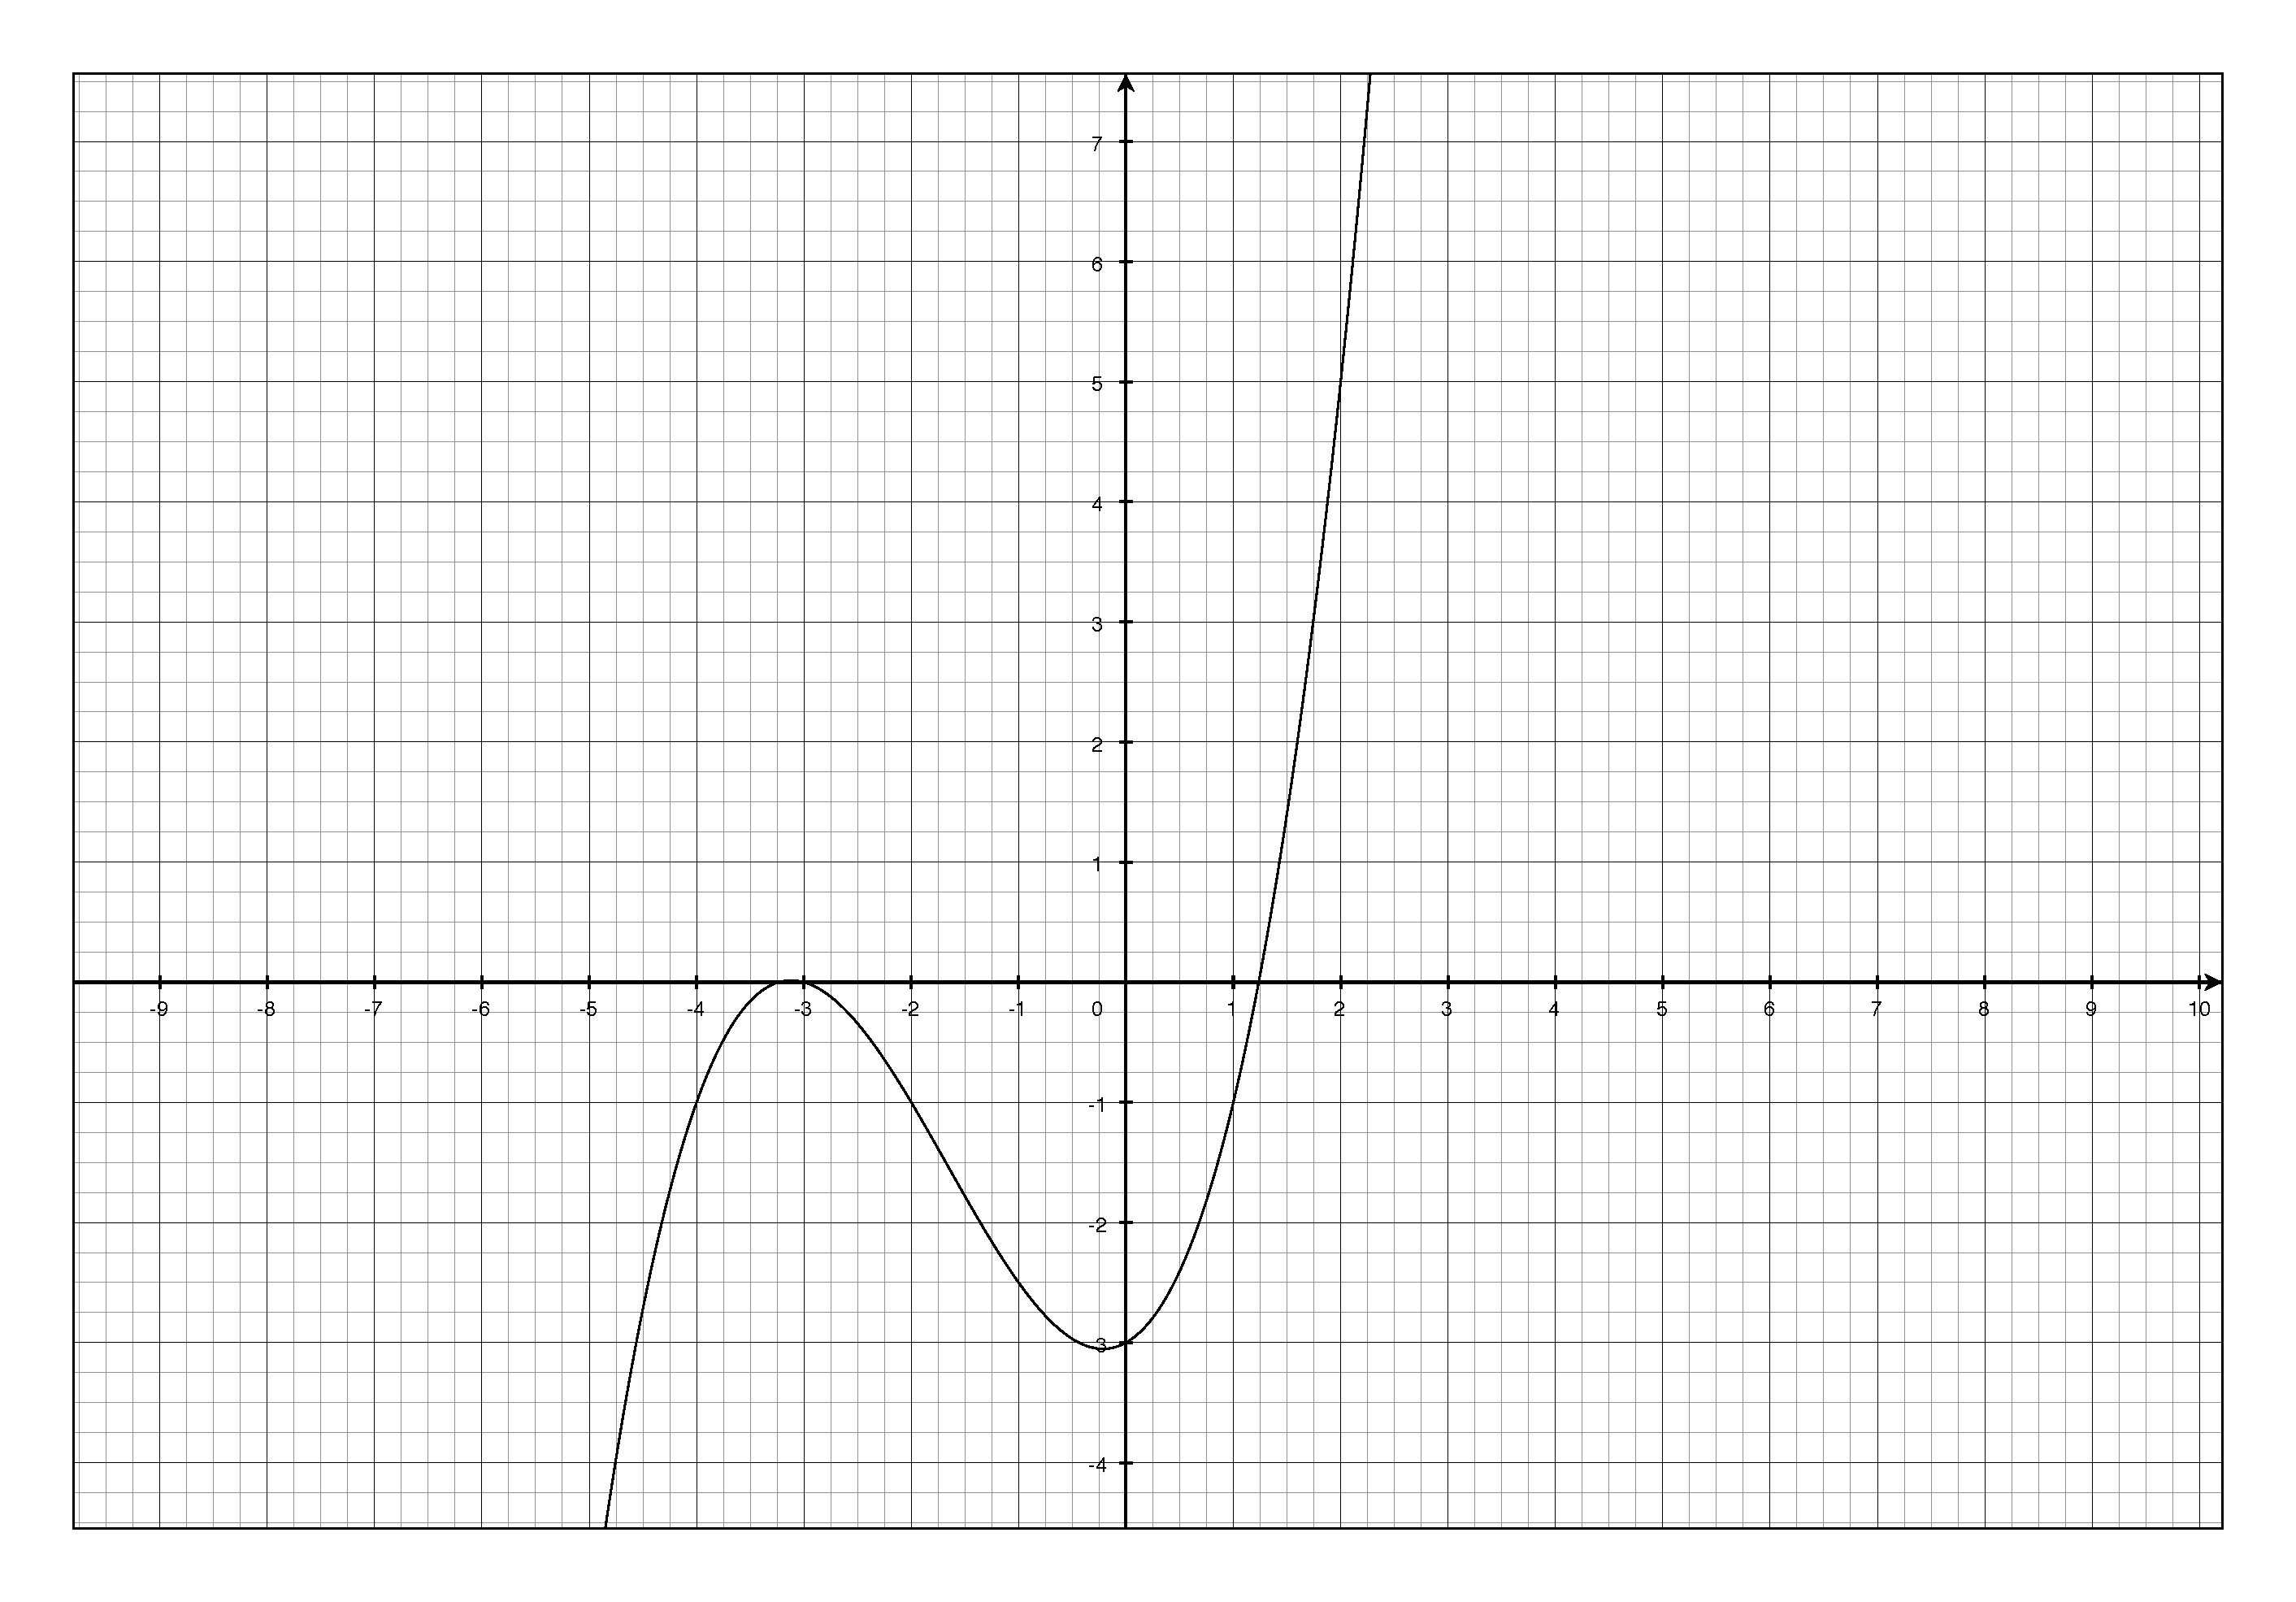
\includegraphics[width=7cm,height=5cm]{1.8-19-e.eps}
%   \caption{$y = f(x+2) - 1$}
% \end{figure}

% \item[f]
% \begin{figure}[H]
%   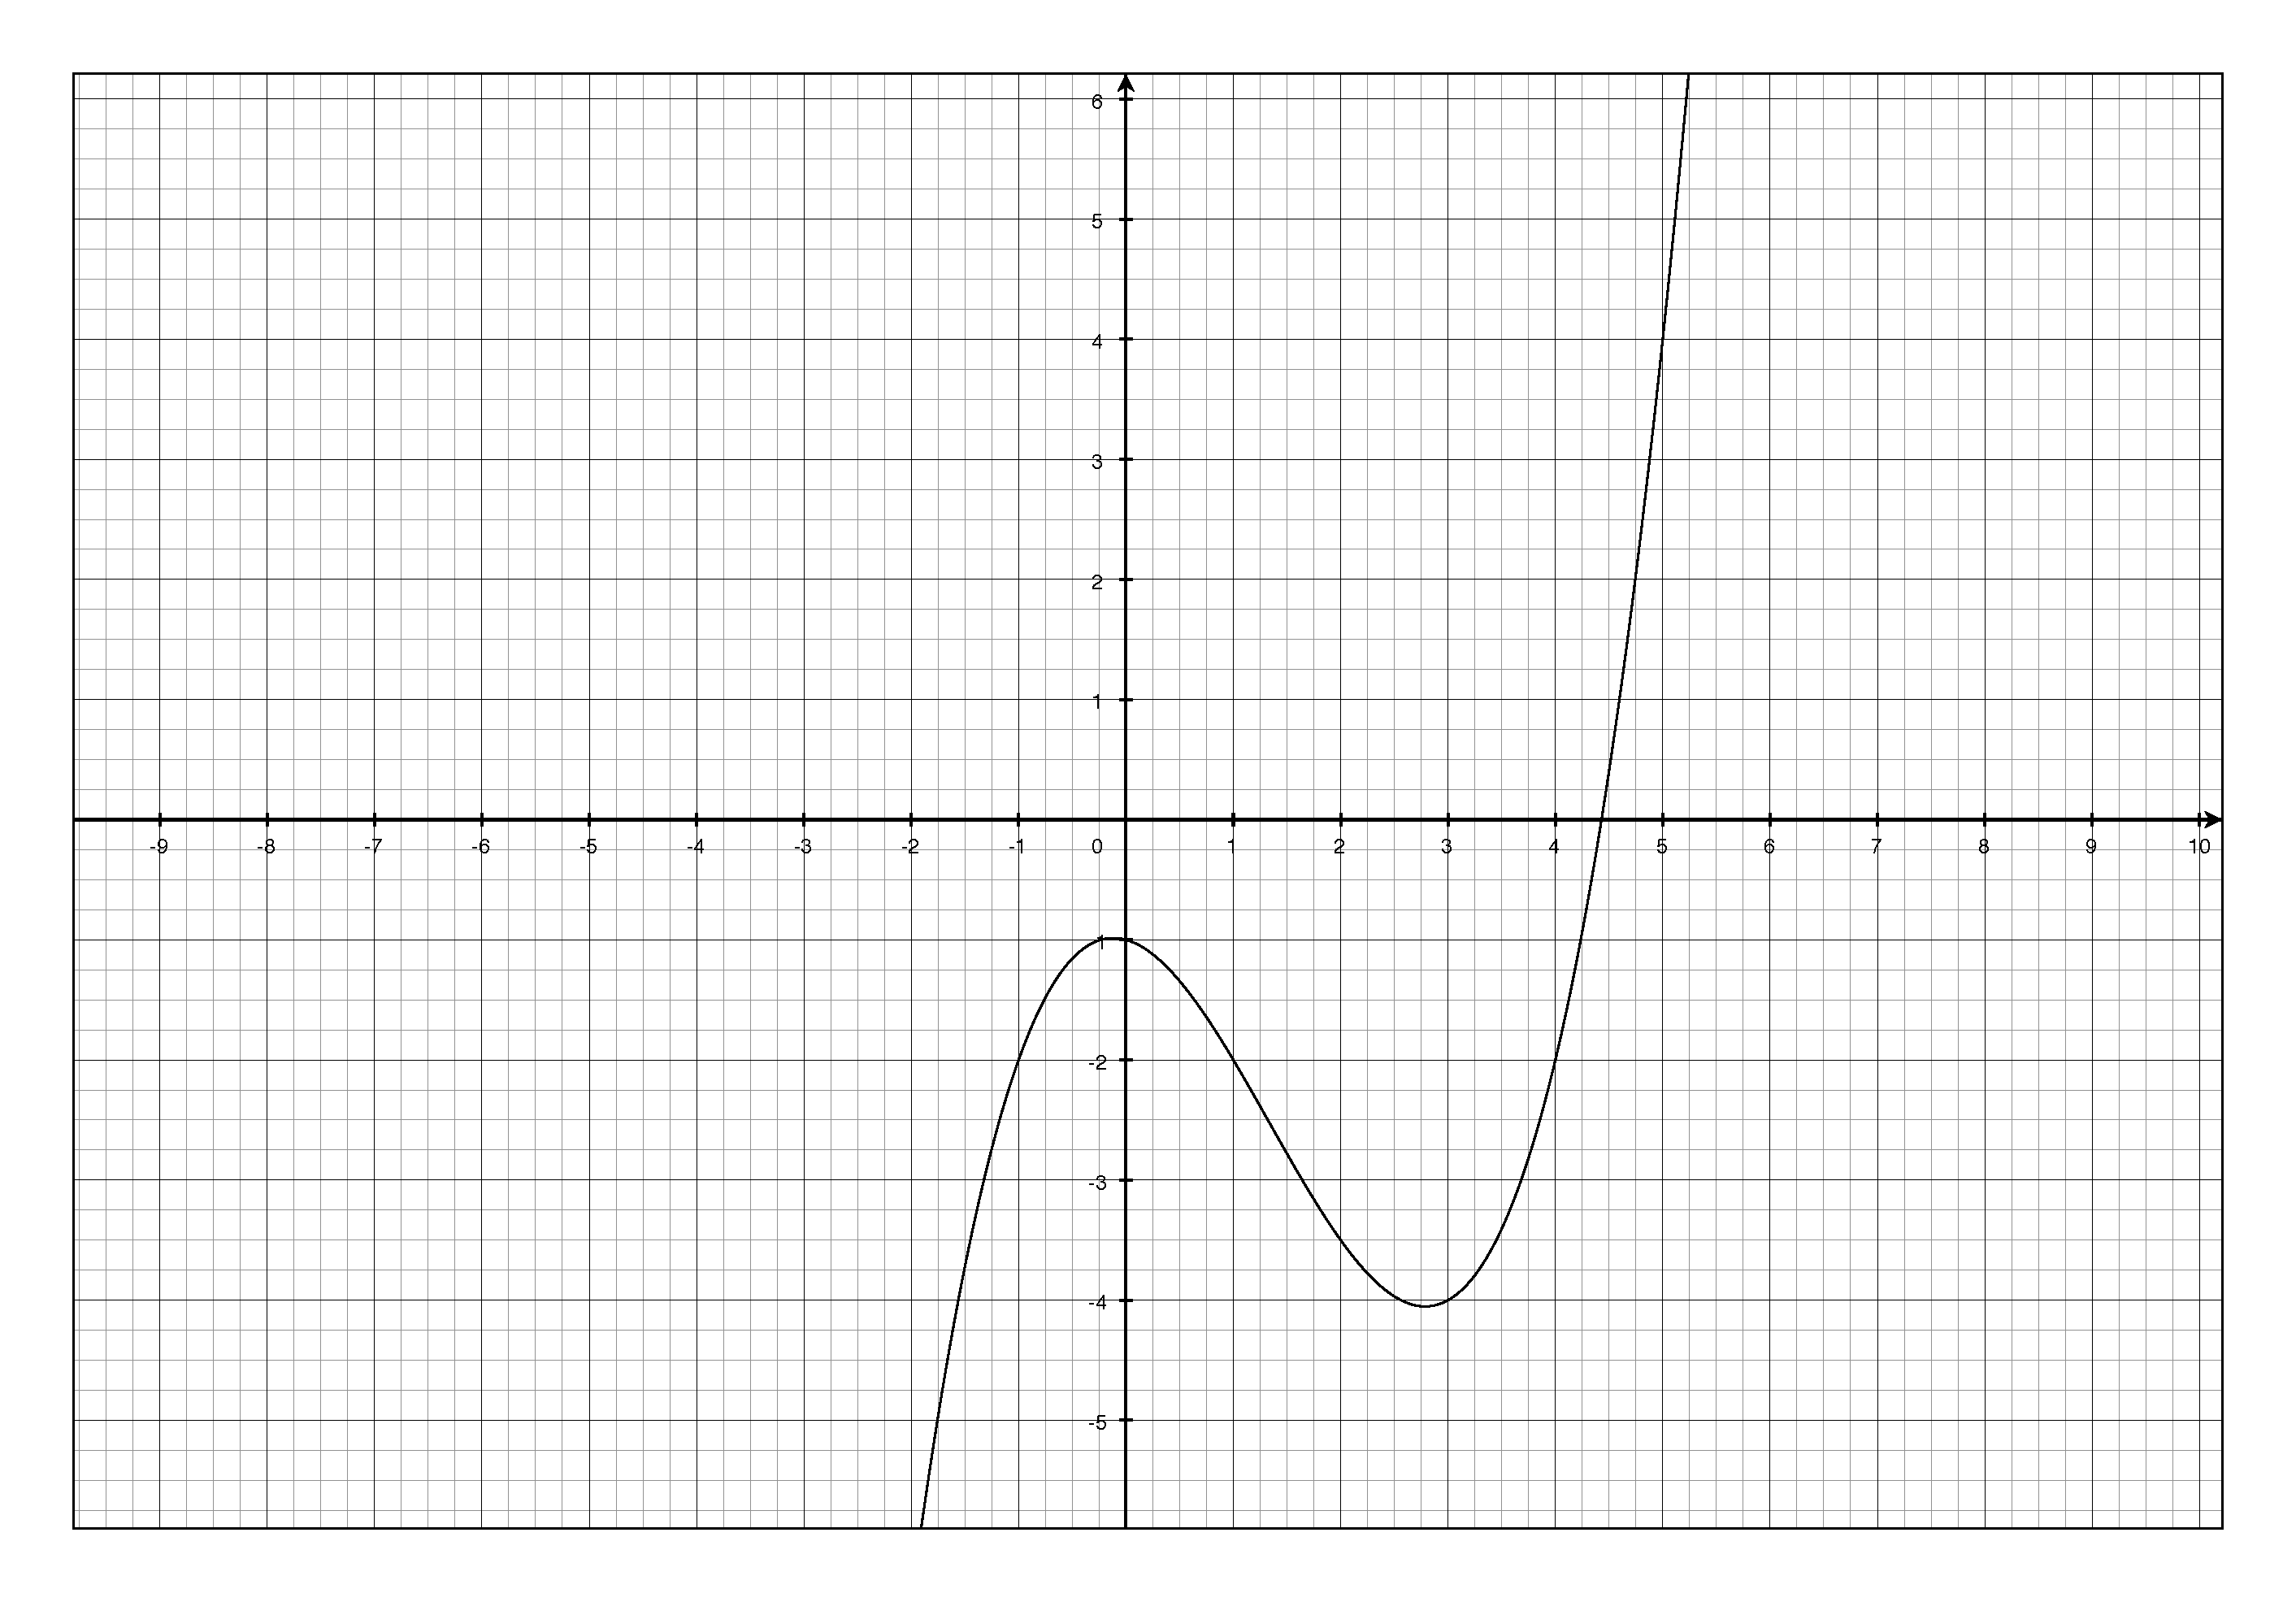
\includegraphics[width=7cm,height=5cm]{1.8-19-f.eps}
%   \caption{$y = f(x-1) - 2$}
% \end{figure}


% \end{itemize}

\item[21]
See the back of the book.

\item[23]
\begin{itemize}
\item[a]

If $(1, 1)$ is on the graph, $f(1) = 1$ and:
\begin{align*}
  a \cdot 1^2 + b \cdot 1 + c &= 1 \\
  a + b + c &= 1
\end{align*}

\item[b]
If the y-intercept is 6, $(0, 6)$ is on the graph, $f(0) = 6$ and:
\begin{align*}
  a \cdot 0^2 + b \cdot 0 + c &= 6 \\
  c &= 6
\end{align*}

\item[c]
If $(1, 1)$ is the vertex, we can get two equations.  For the x-coordinate:

\begin{align*}
  - \frac{b}{2a} &= 1 \\
  b &= -2a
\end{align*}

and for the y-coordinate:
\[
  \frac{4ac - b^2}{4a} = 1
\]

\item[d]

If all of the conditions are satisfied, we can figure out what $a$, $b$, and $c$ are using three of the equations.  It's
easiest to use the three simplest equations, which are:

\begin{align*}
  a+b+c &= 1 \\
  c &= 6 \\
  b &= -2a \\  
\end{align*}

If we substitute the second two equations into the first one, we get an equation with only $a$ in it:
\begin{align*}
  a-2a+6 &= 1 \\
  -a &= -5 \\
  a &= 5 \\
\end{align*}

We can plug the value for $a$ in the second equation to get $b$:
\begin{align*}
  b &= -2a \\
    &= -2(5) \\
    &= -10 \\
\end{align*}

Now we have $a$, $b$, and $c$, so we the equation must be:
\[
  f(x) = 5x^2 - 10x + 6
\]

We can check to see if all the conditions are satisfied.  

To check the vertex, we can complete the square:
\begin{align*}
  f(x) &= 5x^2 - 10x + 6 \\
       &= 5(x^2 - 2x + \frac{6}{5}) \\
       &= 5(x^2 - 2x + 1 - 1 + \frac{6}{5}) \\
       &= 5((x- 1)^2 + \frac{1}{5}) \\
       &= 5(x- 1)^2 + 1 \\
\end{align*}

So the vertex is $(1, 1)$.

To check the y-intercept:
\[
  f(0) = 5(0) - 10(0) + 6 = 6
\]

And since $(1, 1)$ is the vertex, $(1, 1)$ is also on the graph.

\end{itemize}

\item[30]

\begin{itemize}

\item[a]
\begin{align*}
  P(x) &= -x^2 + 200x \\
       &= -(x^2 - 200x) \\
       &= -(x^2 - 200x + 10000 - 10000) \\
       &= -((x - 100)^2 - 10000) \\
       &= -(x - 100)^2 + 10000 \\
\end{align*}

So the vertex is at $(100, 10000)$ and the parabola is inverted because of the negative sign.

Knowing the x-intercepts would also be helpful.  To find them we just need to find the values where $P(x)$ is 0:

\begin{align*}
   -x^2 + 200x &= 0 \\
   x^2 - 200x &= 0 \\
   x(x - 200) &= 0 \\
\end{align*}

So the x-intercepts are at $(0, 0)$ and $(200, 0)$.

Now we have enough information to draw the graph.  To fit everything in, I had to use a different scale for
the x and y axes.

\begin{figure}[H]
  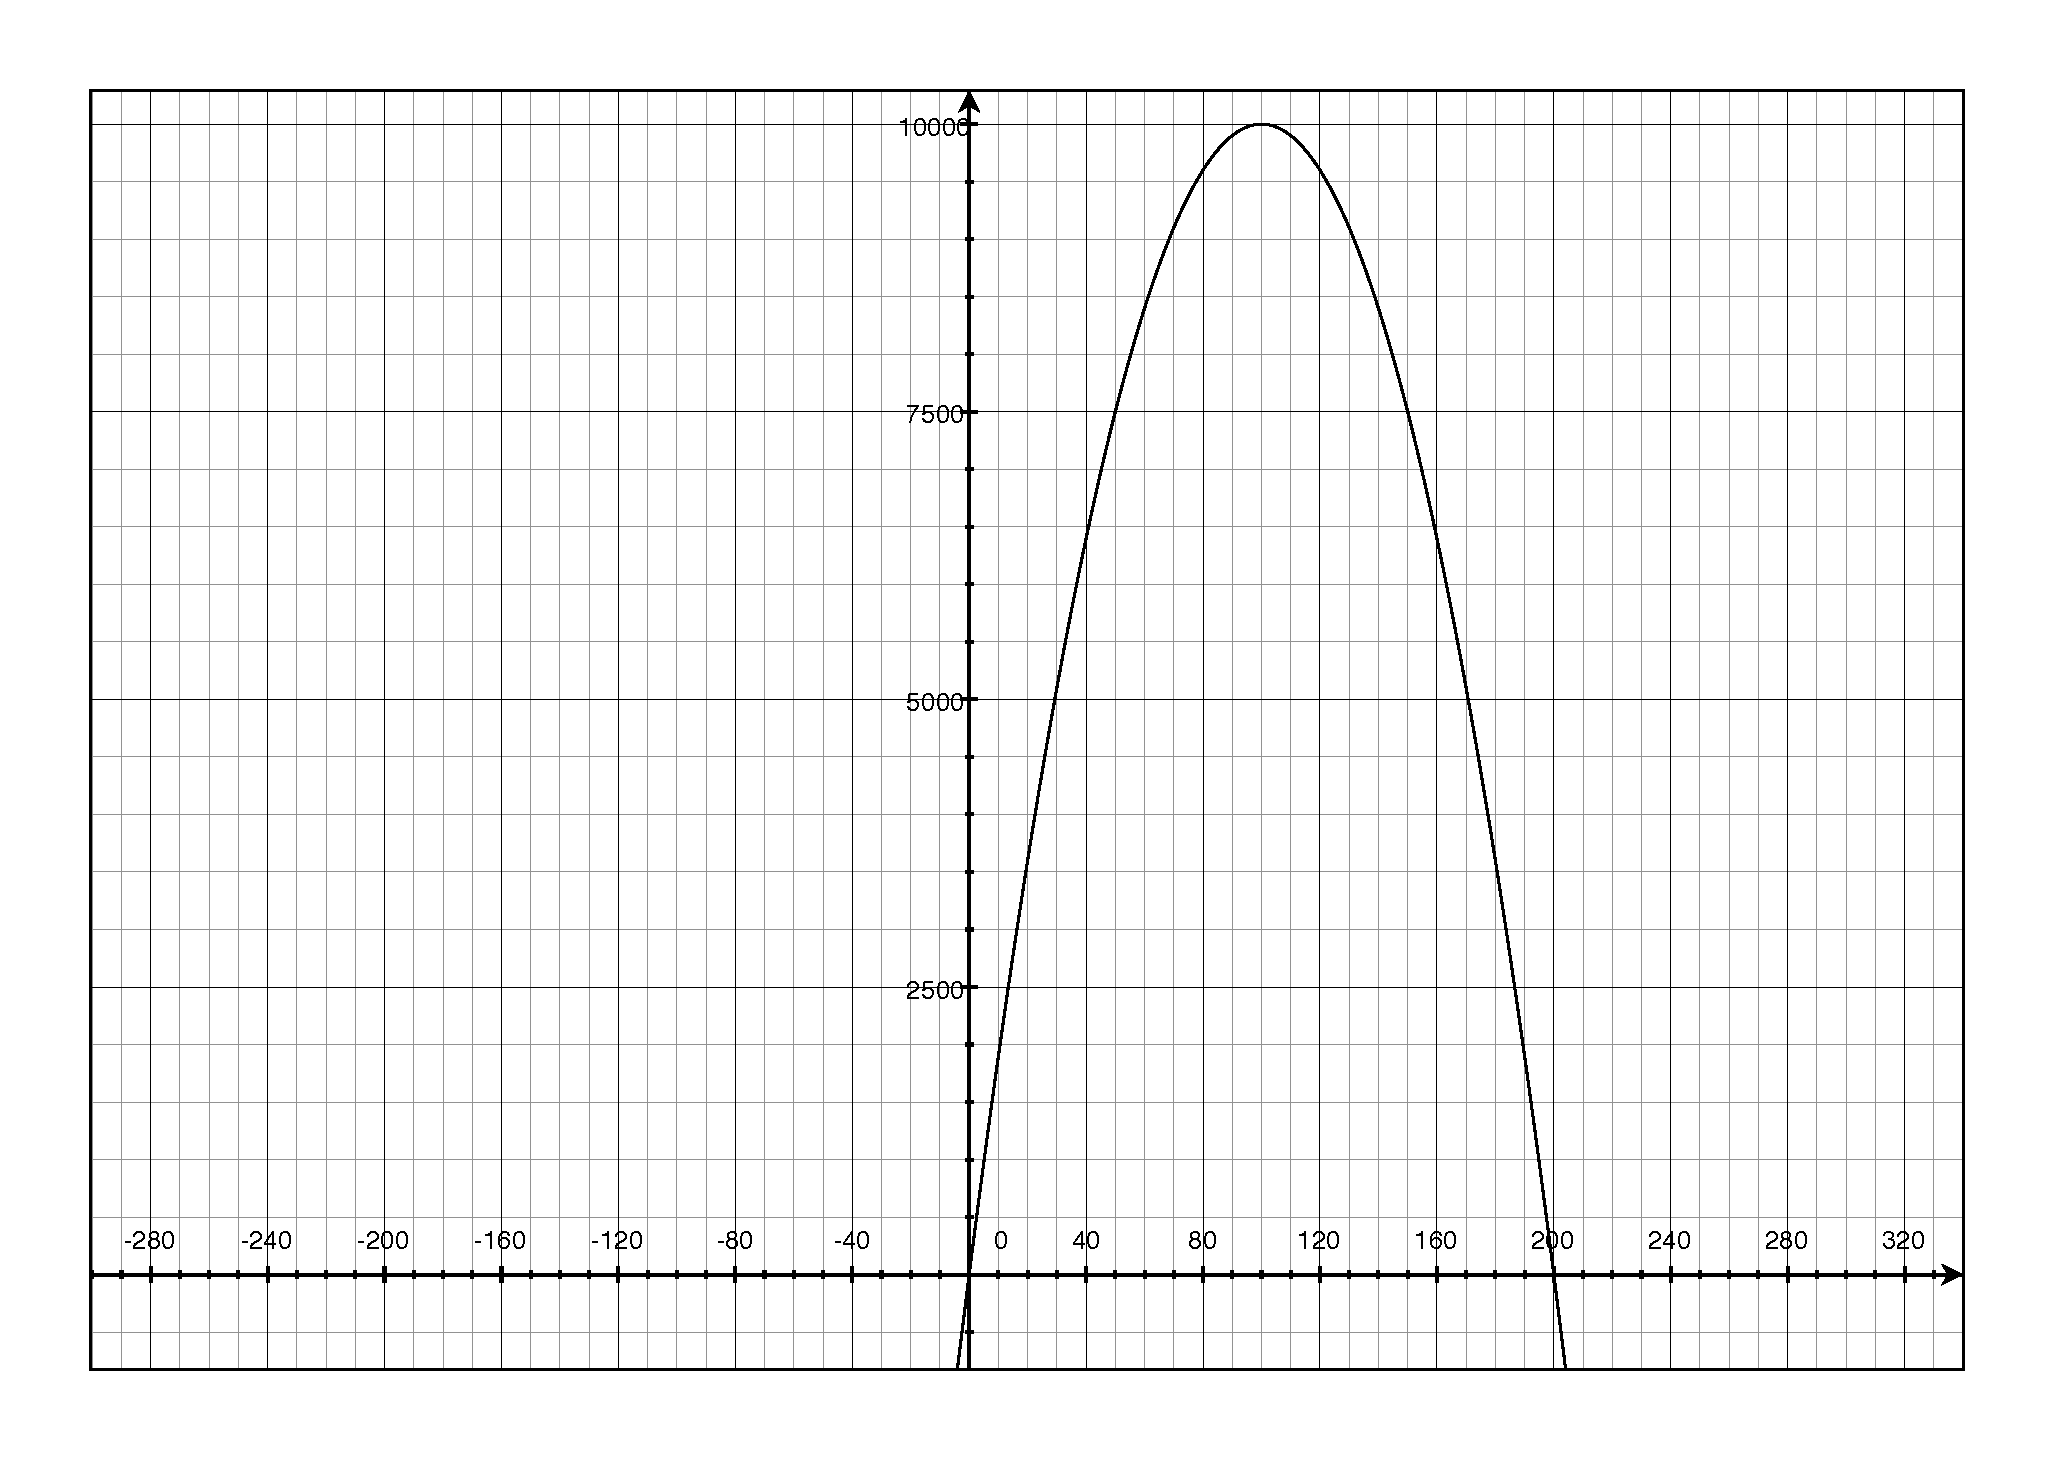
\includegraphics[width=7cm,height=5cm]{1.8-30.eps}
\end{figure}

\item[b]
The maximum profit occurs at the vertex which is 100 units.  For this many units, there is \$10,000 profit.

\item[c]
\begin{align*}
  P(x+h) &= 200(x+h) - (x+h)^2 \\
  &= 200x + 200h - x^2 - 2xh - h^2 \\
\end{align*}

The difference quotient is:
\begin{align*}
  \frac{P(x+h) - P(x)}{h} &= \frac{200x + 200h - x^2 - 2xh - h^2 - (200x - x^2)}{h} \\
  &= \frac{200x + 200h - x^2 - 2xh - h^2 - 200x + x^2)}{h} \\
  &= \frac{200h - 2xh - h^2}{h} \\
  &= \frac{\cancel{h}(200 - 2x - h)}{\cancel{h}} \\
  &= 200 - 2x - h \\
\end{align*}

If $h$ gets close to zero, it disappears from the equation and we are left with $200 - 2x$.

When $x<100$, $200 - 2x$ is positive, so making more units will help us make more money.  When $x>100$, $200-2x$ is negative
so making more units will cause us to make less money.  This agrees with part {\em b} where we found that making 100
units produced the maximum profit.

\end{itemize}

\end{itemize}

\fi

\subsection{Other Problems}

\subsubsection{Linear Functions}

For questions \ref{si:first} - \ref{si:last} find the slope-intercept forms of the equations of the lines through the
given point (a) parallel to the given line and (b) perpendicular to the given line.

\begin{questions}
 
\question
\label{si:first}
point: $(2, 1)$ and line $4x-2y = 3$

\begin{parts}

\part
\begin{solution}[1cm]
First put the original equation in slope/intercept form so we know the slope:
\begin{align*}
  4x - 2y &= 3 \\
  -2y &= -4x + 3 \\
  y &= 2x - \frac{3}{2} \\
\end{align*}

The parallel line will have the same slope but a different y-intercept:
\begin{align*}
  y &= 2x + b \\
  1 &= 2(2) + b \\
  b &= -3 \\
\end{align*}

So the equation for the parallel line is: $f(x) = 2x - 3$

The perpendicular line will have the negative reciprocal slope and a different y-intercept:
\begin{align*}
  y &= - \frac{1}{2}x + b \\
  1 &= - \frac{1}{2} (2) + b \\
  1 &= -1 + b \\
  b &= 1 \\
\end{align*}

So the equation for the parallel line is: $f(x) = - \frac{1}{2}x + 2$

Here are all three lines:
\begin{figure}[H]
  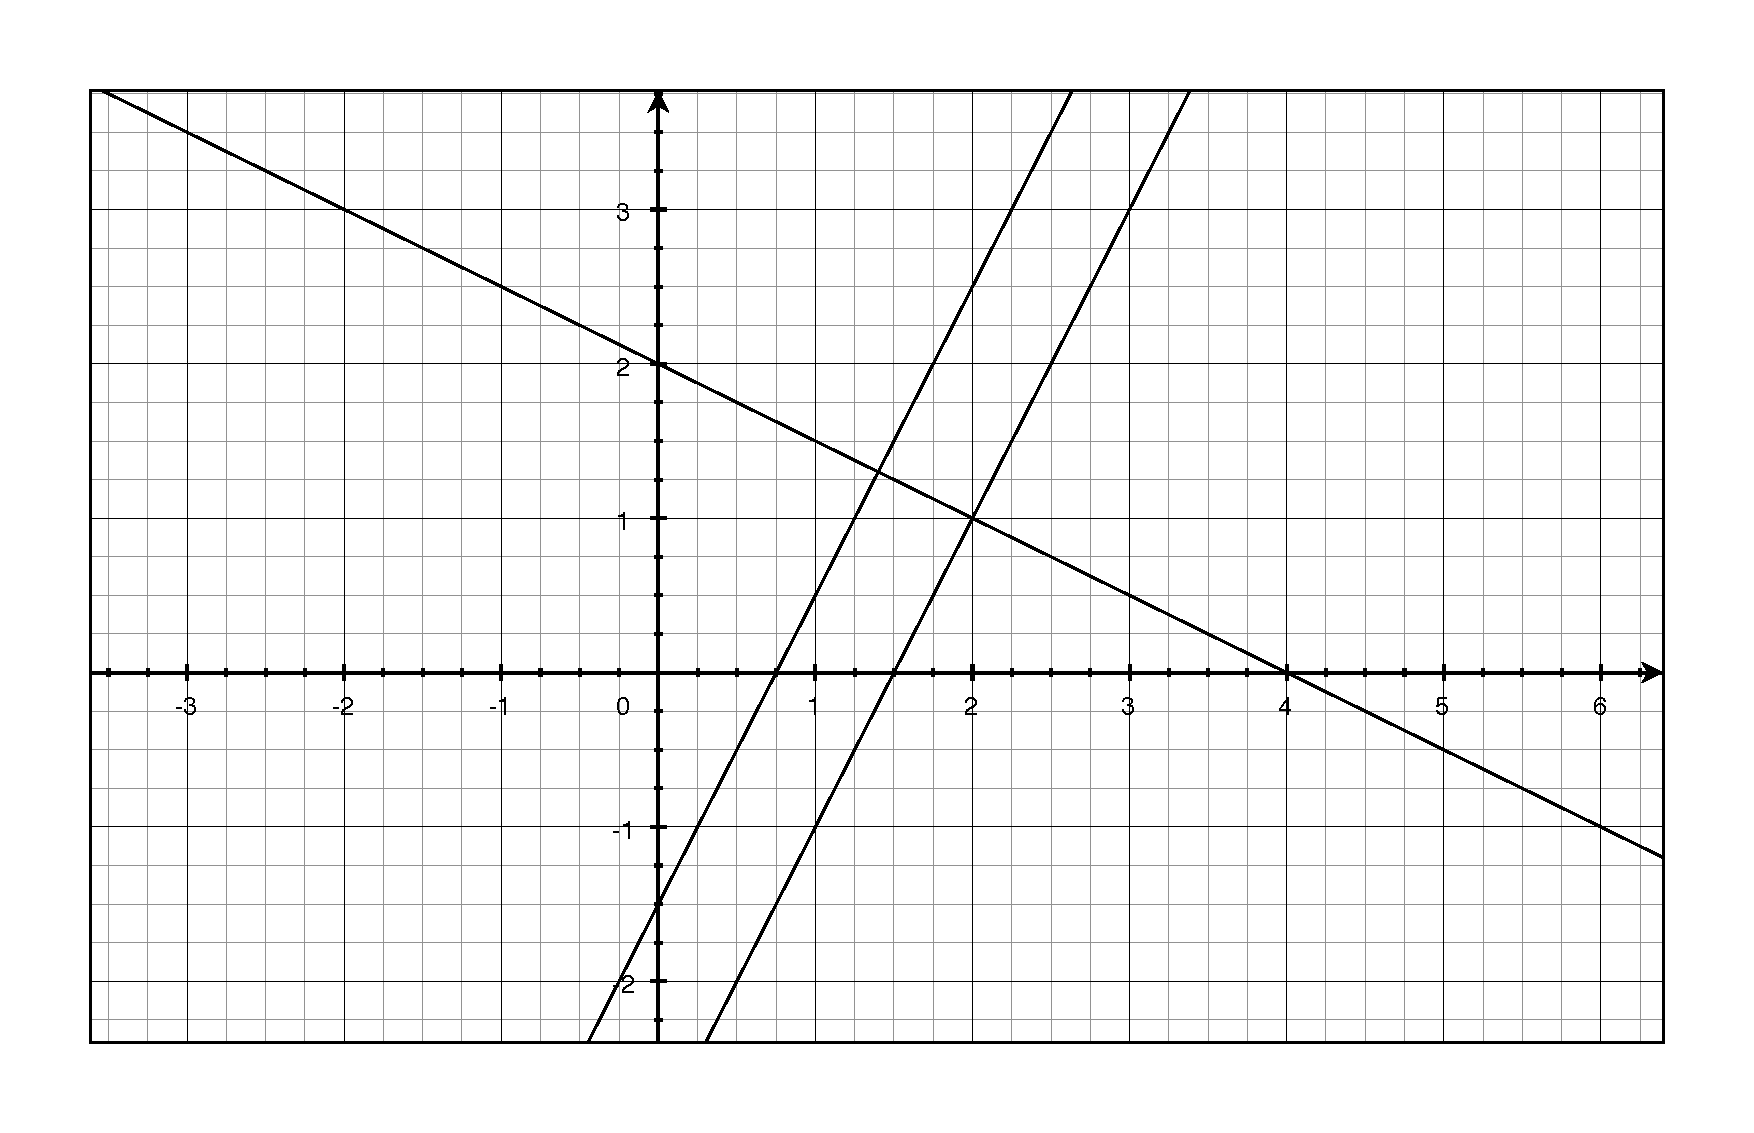
\includegraphics[width=7cm,height=5cm]{linear-1}
\end{figure}

\end{solution}

\end{parts}

\question
point: $\left( \dfrac{7}{8}, \dfrac{3}{4} \right)$ and line $5x + 3y = 0$

\begin{solution}[1cm]
First put the original equation in slope/intercept form so we know the slope:
\begin{align*}
  5x + 3y &= 0 \\
  3y &= -5x \\
  y &= -\frac{5}{3} x \\
\end{align*}

The parallel line will have the same slope but a different y-intercept:
\begin{align*}
  y &= -\frac{5}{3} x + b \\
  \frac{3}{4} &= -\frac{5}{3} \cdot \frac{7}{8} + b \\
  \frac{3}{4} &= -\frac{35}{24}  + b \\
  b &= \frac{3}{4} + \frac{35}{24} \\
  b &= \frac{18}{24} + \frac{35}{24} \\
  b &= \frac{53}{24} \\
\end{align*}

So the equation for the parallel line is: $f(x) = -\dfrac{5}{3} x + \dfrac{53}{24}$

The perpendicular line will have the negative reciprocal slope and a different y-intercept:
\begin{align*}
  y &= \frac{3}{5}x + b \\
  \frac{3}{4} &= \frac{3}{5} \cdot \frac{7}{8} + b \\
  \frac{3}{4} &= \frac{21}{40} + b \\
  b &= \frac{3}{4} - \frac{21}{40} \\
  b &= \frac{30}{40} - \frac{21}{40} \\
  b &= \frac{9}{40} \\
\end{align*}

So the equation for the perpendicular line is: $f(x) = \dfrac{3}{5}x + \dfrac{9}{40}$

\end{solution}

\question
\label{si:last}
point: $(-1, 0)$ and line $y = -3$

\begin{solution}
The line $y = -3$ is a horizontal line.  The parallel line through $(-1, 0)$ is the x-axis or $y = 0$.  The
perpendicular line through $(-1, 0)$ is the vertical line at $x = -1$.
\end{solution}

\question 
A business purchases a piece of equipment for \$25,000.  After 10 years, the equipment will have to be replaced.  Its
value at that time is expected to the \$2,000.  Write a linear function $V(t)$ giving the value of the equipment during
the 10 years it will be used.

\begin{solution}

There is a typo in the last sentence, which should have read ``during the 10 years it will be used.''

We start out with two points.  At time 0, the value is \$25,000.  At time 10, the value is \$2,000.  So the two points
are $(0, 25,000)$ and $(10, 2,000)$.

The slope is:
\[
  m = \frac{25,000 - 2,000}{0 - 10} = \frac{23,000}{10} = -2,300
\]

The y-intercept is one of the original points, so the function is:
\[
   V(t) = -2,300t + 25,000
\]

\end{solution}


\subsubsection{Transformations}

\question
Use the graph of $f(x) = x^2$ to write an equation for each function whose graph is shown.
\begin{parts}

\part

\begin{solution}
The graph is shifted down by 2, so the function is $f(x) = x^2 - 2$

\begin{figure}[H]
  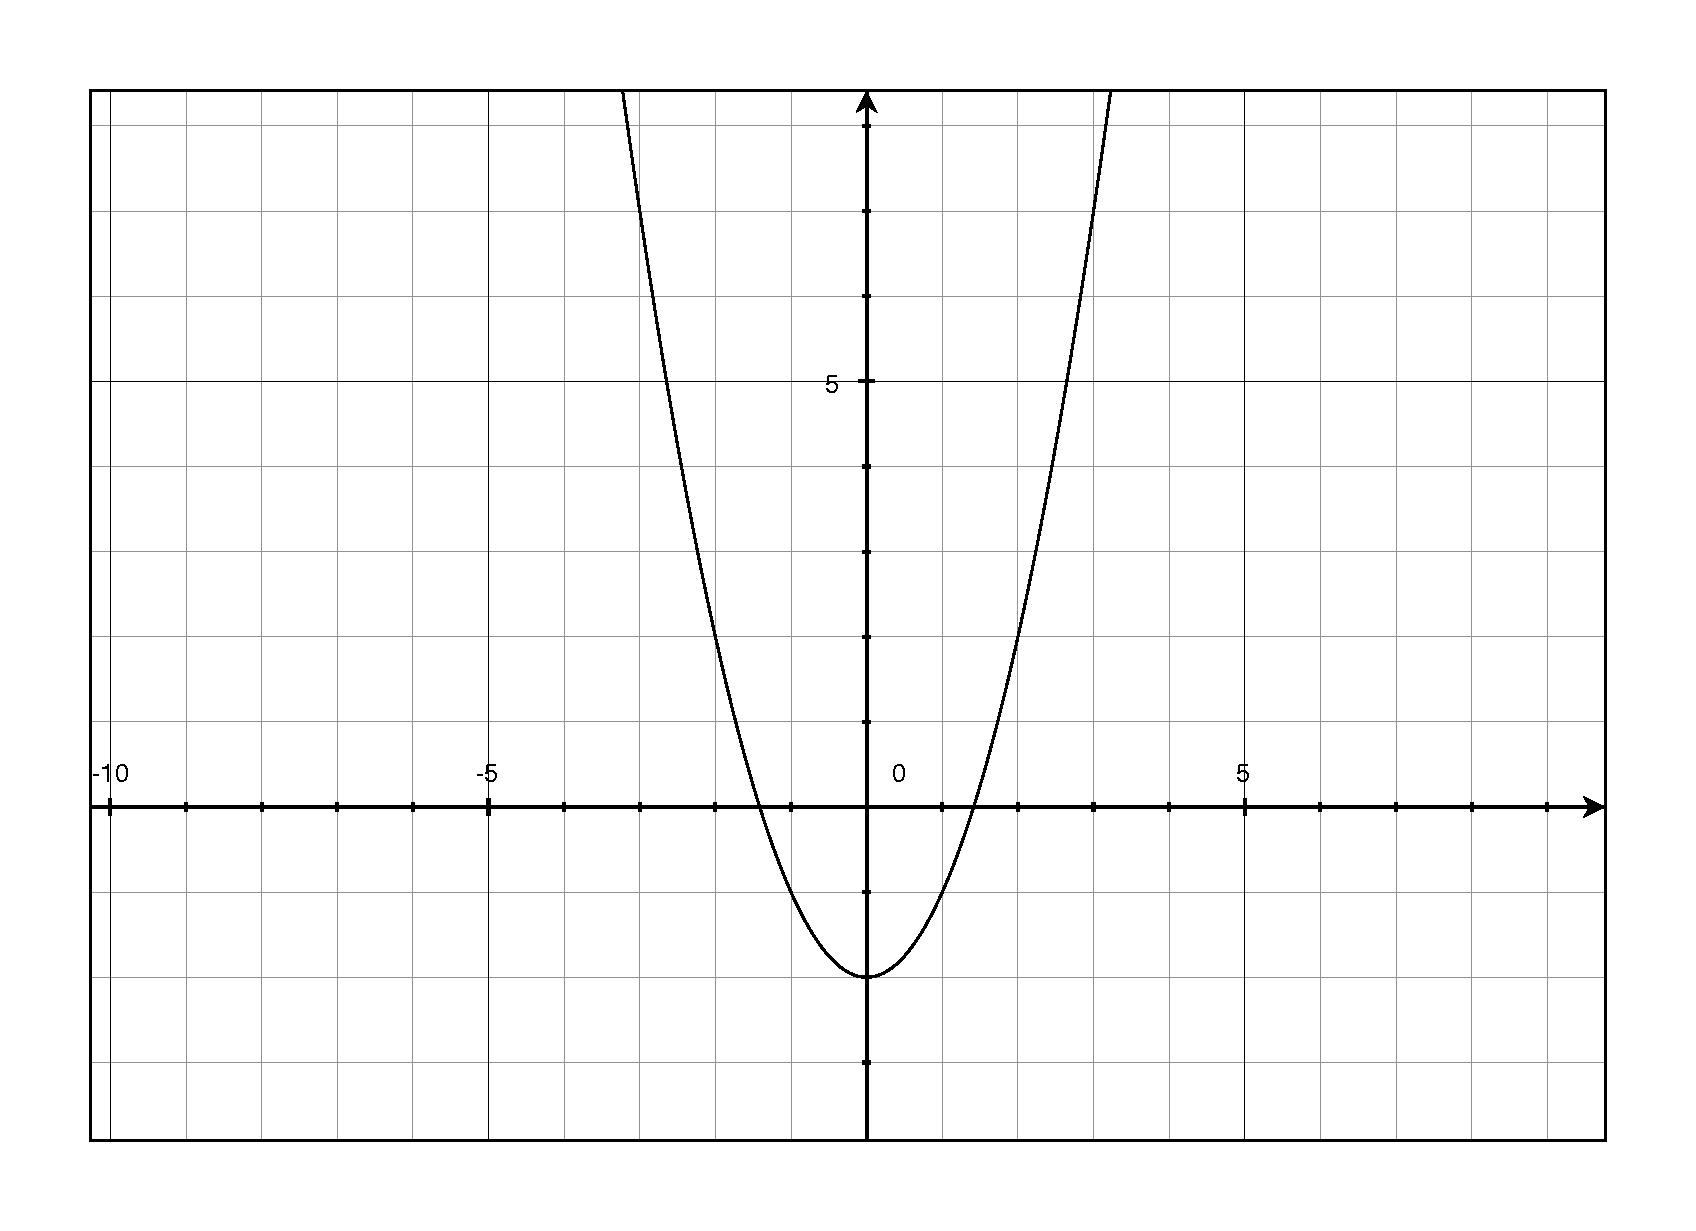
\includegraphics[width=7cm,height=5cm]{transformation-a}
\end{figure}

\end{solution}

\part

\begin{solution}
The graph is inverted and shifted up 1 and left 1, so the function is $f(x) = -(x+1)^2 + 1$

\begin{figure}[H]
  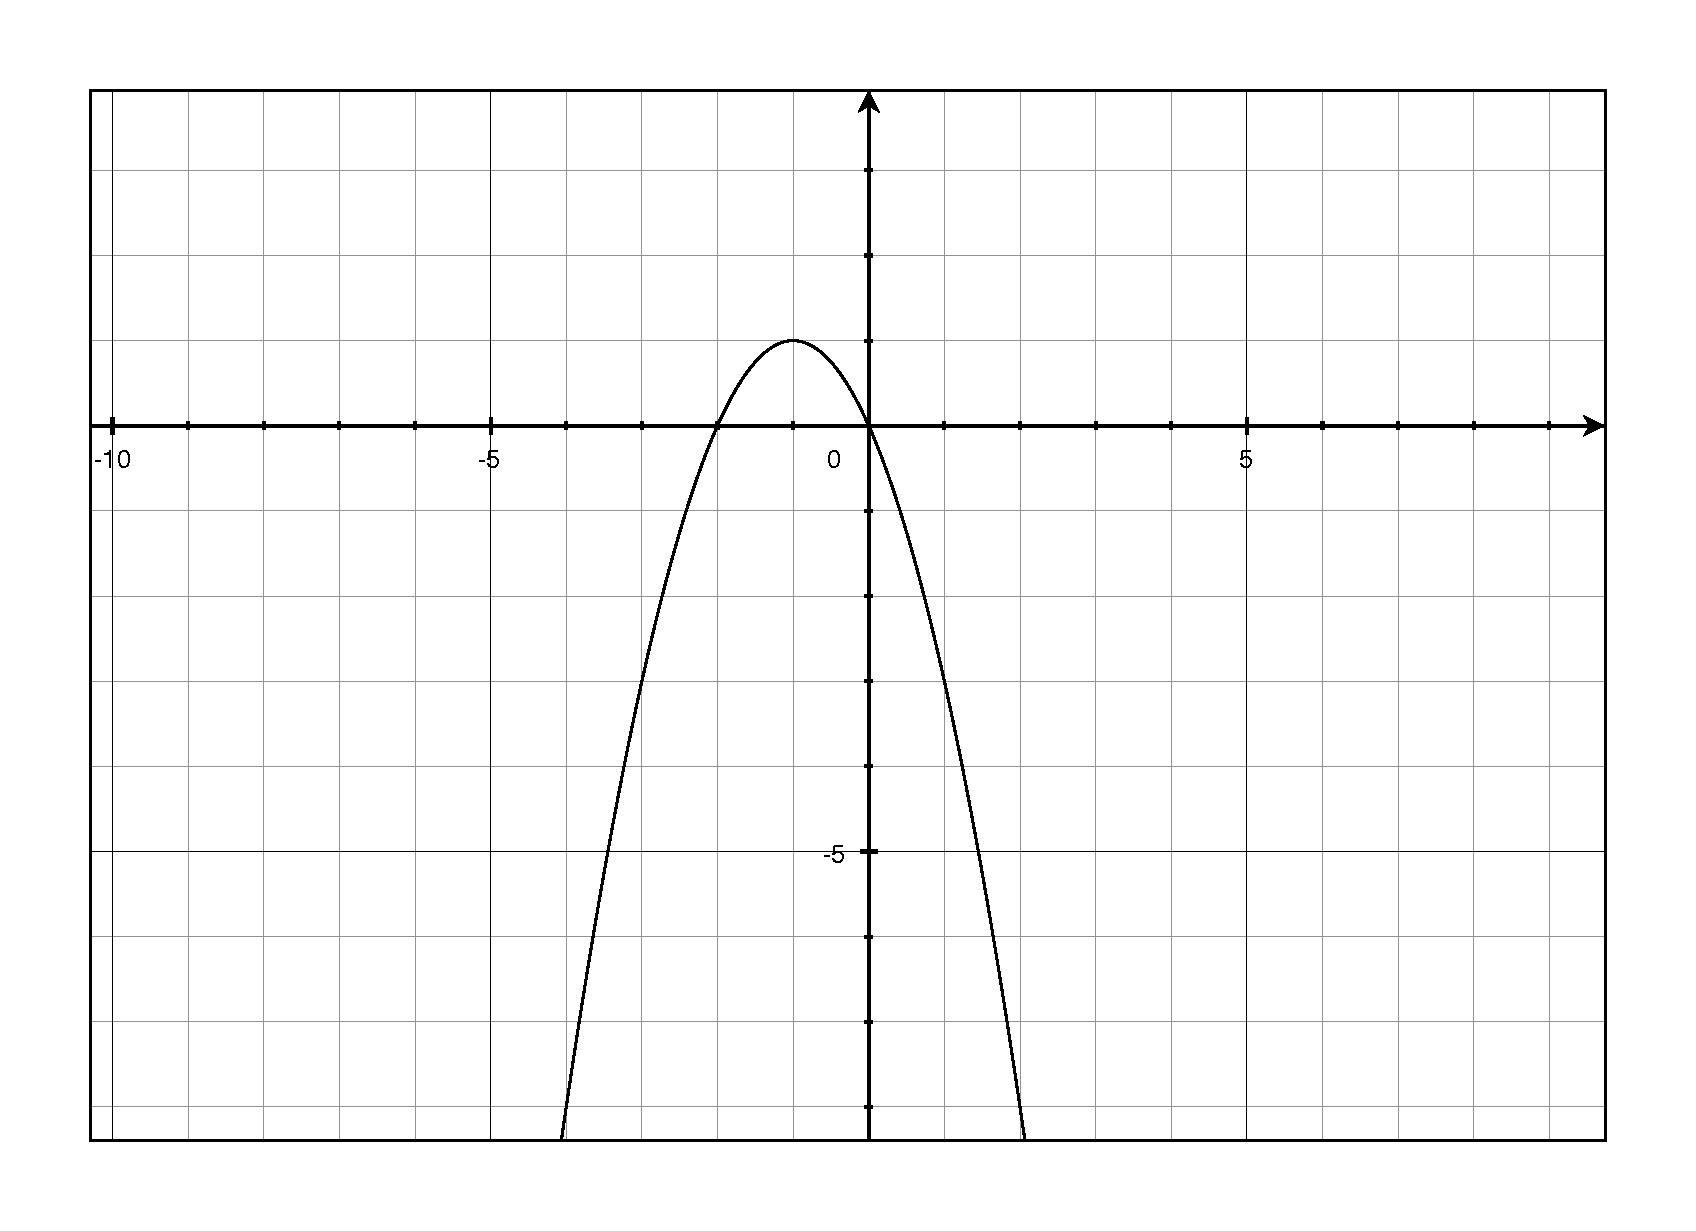
\includegraphics[width=7cm,height=5cm]{transformation-b}
\end{figure}

\end{solution}

\part
\begin{solution}
The graph is inverted and shifted up 3 and right 2, so the function is $f(x) = -(x-2)^2 + 3$

\begin{figure}[H]
  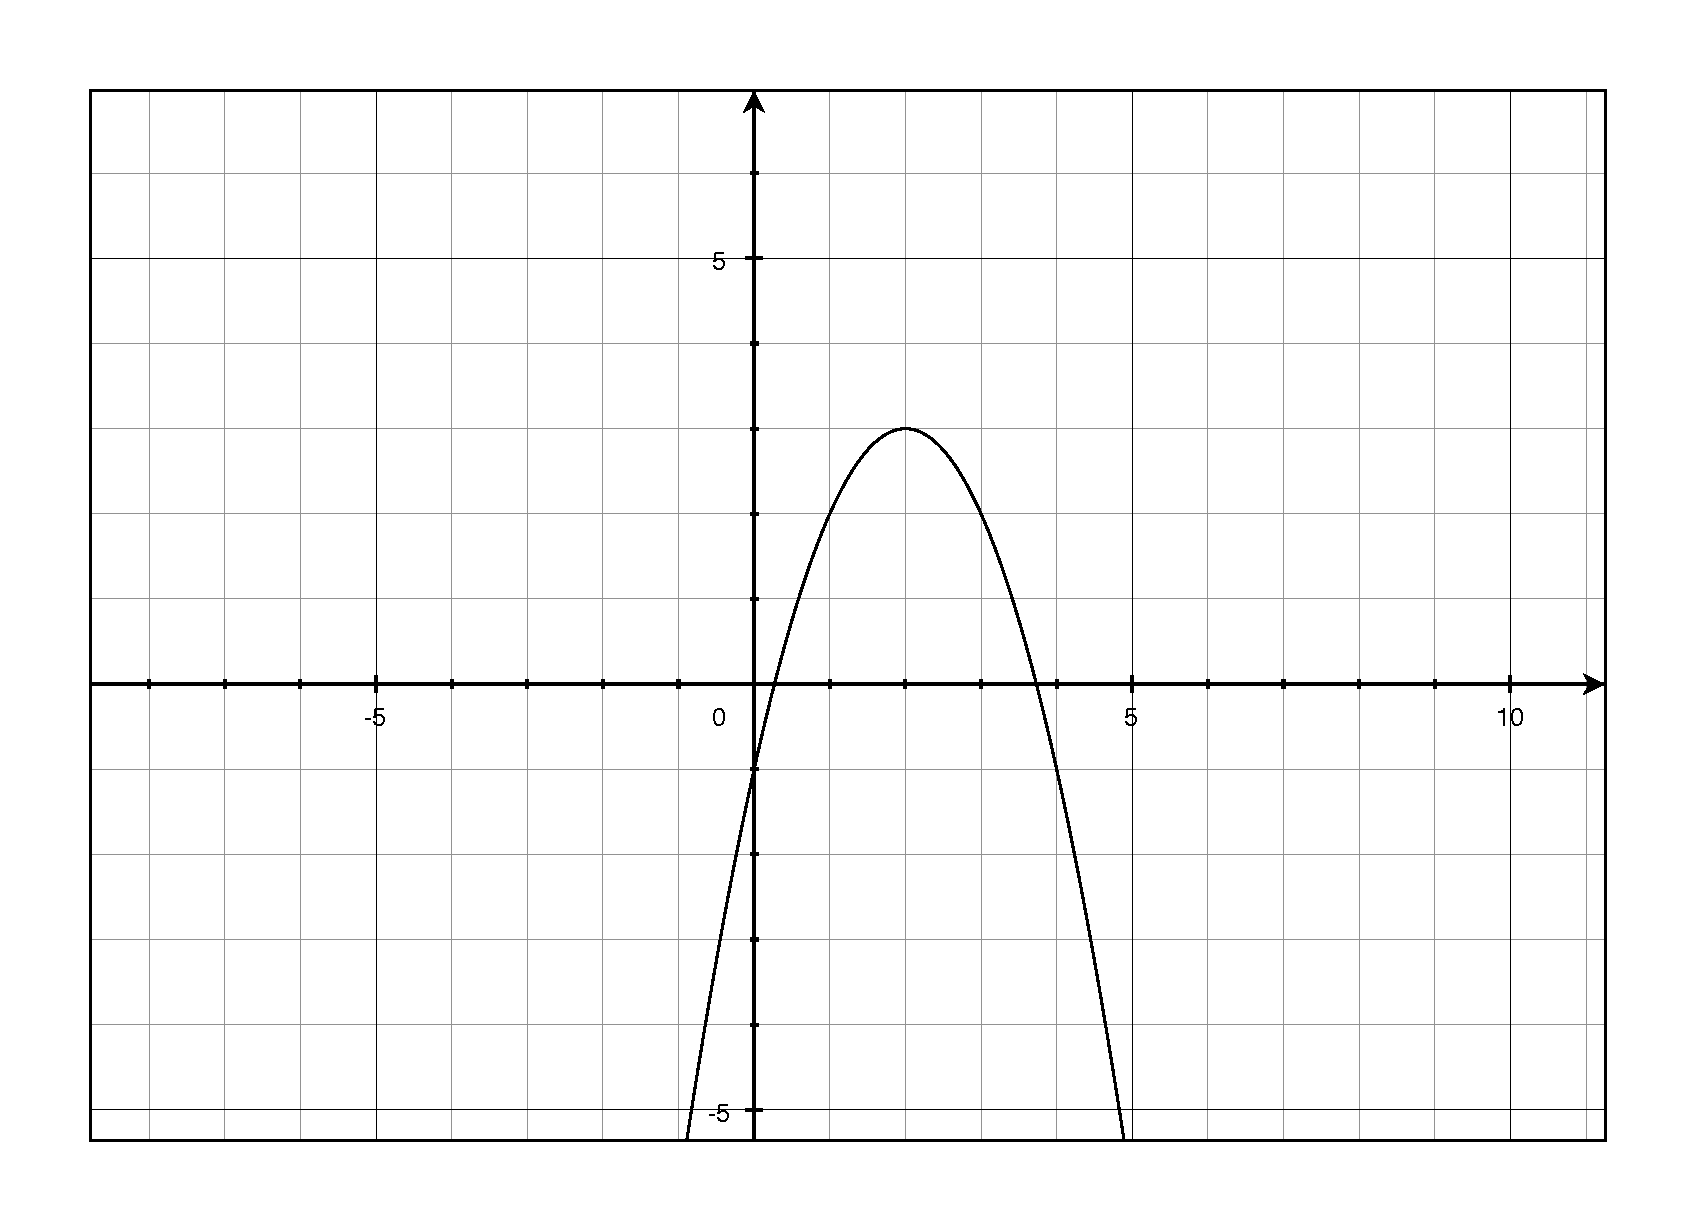
\includegraphics[width=7cm,height=5cm]{transformation-c}
\end{figure}

\end{solution}

\part
\begin{solution}
The graph shifted down 2 and right 3, so the function is $f(x) = (x-3)^2 - 2$

\begin{figure}[H]
  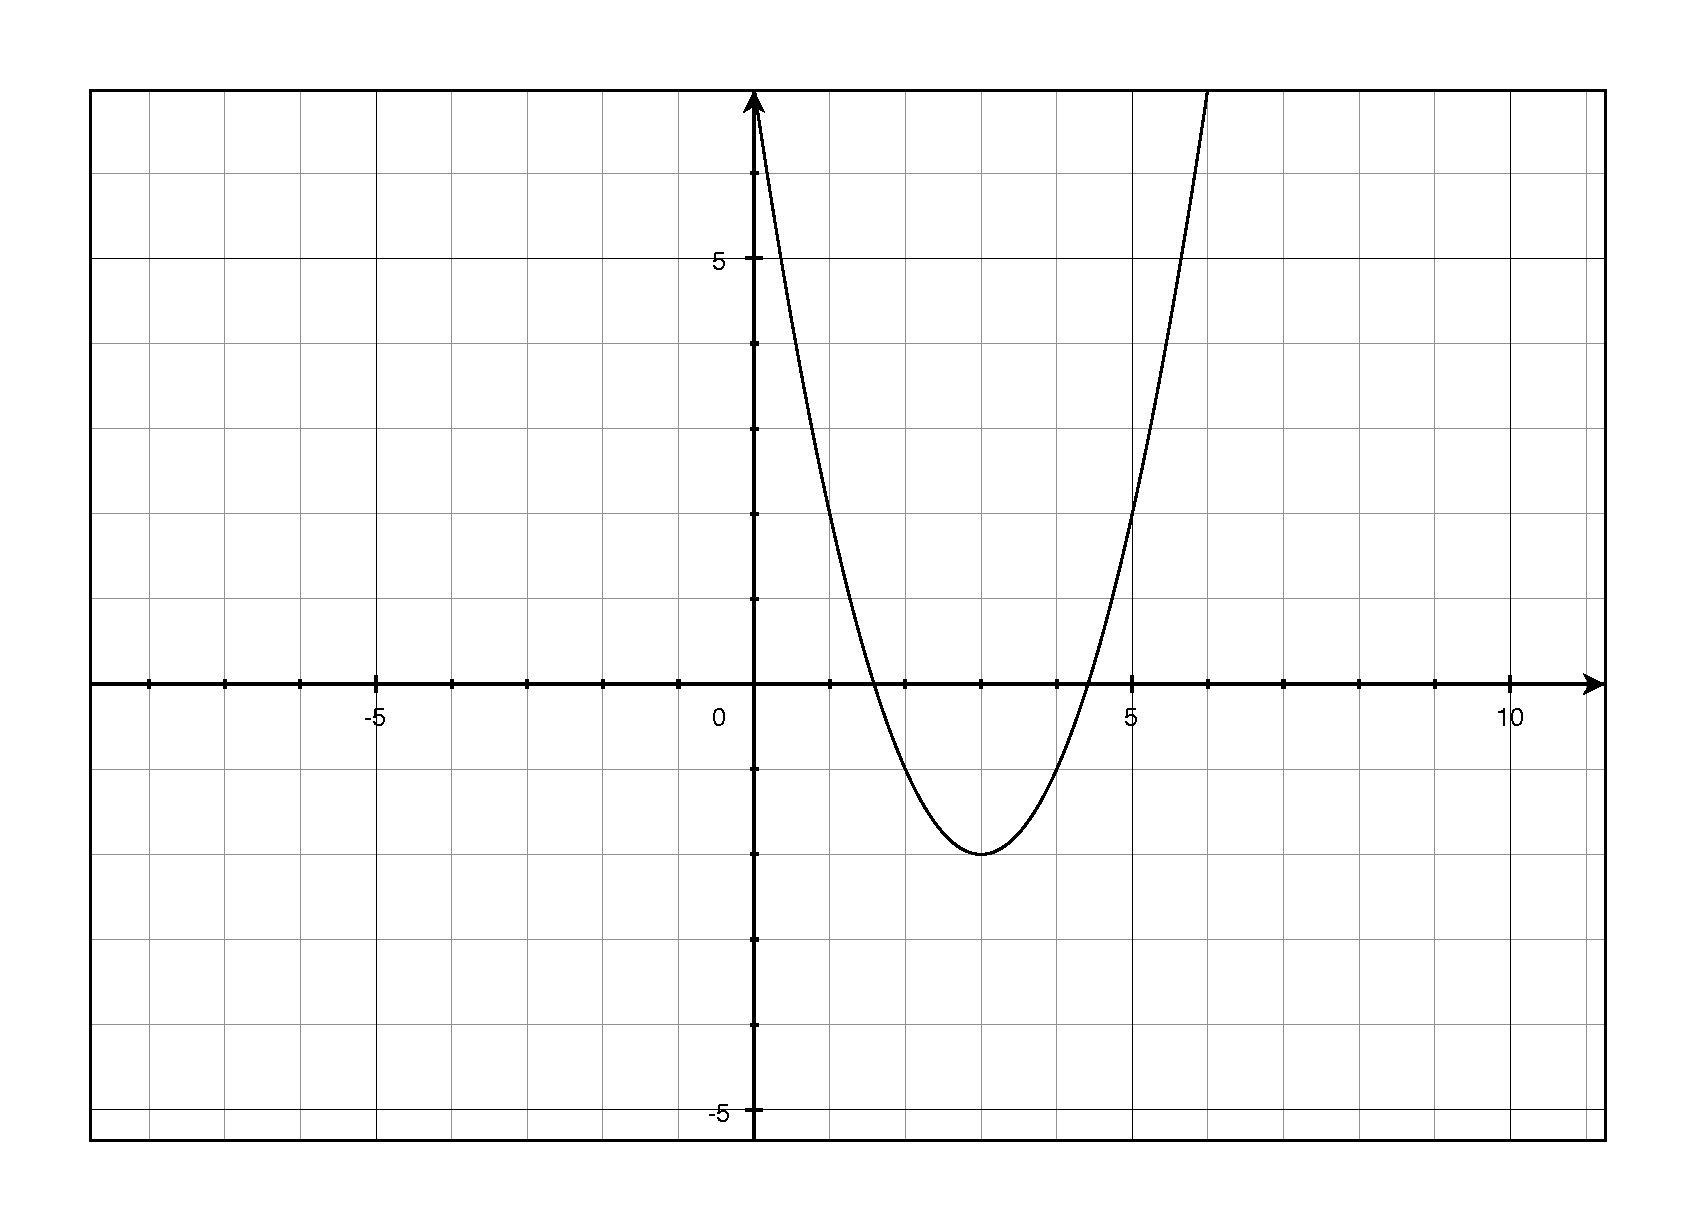
\includegraphics[width=7cm,height=5cm]{transformation-d}
\end{figure}

\end{solution}

\end{parts}

\question
Write an equation for the function that is described by the given characteristics.

\begin{parts}
\part The shape of $f(x) = x^2$ but moved 2 units to the right and 8 units down.

\begin{solution}[1cm]
\[
  g(x) = (x-2)^2 - 8
\]
\end{solution}


\part The shape of $f(x) = |x|$ but moved 1 unit to the left and 7 units down.
\begin{solution}[1cm]
\[
  g(x) = |x+2| - 7
\]
\end{solution}

\part The shape of $f(x) = \sqrt{x}$ but moved 6 units to the left and reflected in the x-axis.

\begin{solution}[1cm]
\[
  g(x) = - \sqrt{x+6}
\]
\end{solution}

\end{parts}

\subsubsection{Quadratic Functions}

\question
Find the quadratic function that has the indicated vertex and whose graph passes through the given point
\begin{parts}
\part Vertex: $(-2, 5)$; Point: $(0, 9)$

\begin{solution}[1cm]

First find an equation using the vertex:
\begin{align*}
  y &= a(x - (-2))^2 + 5 \\
    &= a(x + 2)^2 + 5 \\
\end{align*}

Then use the point to find $a$:
\begin{align*}
  y  &= a(x + 2)^2 + 5 \\
  9  &= a(0 + 2)^2 + 5 \\
  9  &= 4a + 5 \\
  4a  &= 4 \\
  a  &= 1 \\
\end{align*}

So the function is: $f(x) = (x+2)^2 + 5$

\end{solution}

\part Vertex: $(3, 4)$; Point: $(1, 2)$


\begin{solution}[1cm]
First find an equation using the vertex:
\[
  y = a(x -3)^2 + 4
\]

Then use the point to find $a$:
\begin{align*}
  y  &= a(x - 3)^2 + 4 \\
  2  &= a(1 - 3)^2 + 4 \\
  2  &= 4a + 4 \\
  4a &= -2 \\
  a &= - \frac{1}{2}
\end{align*}

So the function is: $f(x) = - \frac{1}{2}(x-3)^2 + 4$

\end{solution}

\end{parts}


\subsection{Extra Credit}

\question

The height (in feet) of a ball thrown by a child is:

\[
  h(x) = - \frac{1}{12} x^2 + 2x + 4
\]

 where $x$ is the horizontal distance (in feet) from the point at which the ball is thrown.

\begin{parts}

\part How high is the ball when it leaves the child's hand?
\begin{solution}
When the ball leaves the child's hand, its $x$ coordinate is 0.  At this time, its height is:

\[
  h(0) = - \frac{1}{12} (0)^2 + 2(0) + 4 = 4
\]

So the ball leaves the child's hand 4 feet from the ground.

\end{solution}
\part What is the maximum height of the ball

\begin{solution}
Because the sign of the $x^2$ coordinate is negative, the parabola is inverted and the maximum height occurs at the
vertex.  The $x$ coordinate of the vertex is:

\[
  x_{max} = \frac{-2}{2 \left(- \cfrac{1}{12} \right) } = 12
\]

At this point, the height will be:
\[
  h(12) = - \frac{1}{12} (12)^2 + 2(12) + 4 = -12 + 24 + 4 = 16
\]

So the maximum height is 16 feet and it occurs after the ball has travelled 12 feet.

\end{solution}

\part How far from the child does the ball strike the ground?
\begin{solution}
When the ball hits the ground, its height is 0.  We can set the height to 0 and solve for the x coordinate:
\begin{align*}
  - \frac{1}{12} x^2 + 2x + 4 &= 0  \\
  -x^2 + 24x + 48 &= 0  \\
  x^2 - 24x - 48 &= 0  \\
\end{align*}

Using the quadratic equation:
\begin{align*}
  x &= \frac{24 \pm \sqrt{(-24)^2 - 4(1)(-48)}}{2} \\
    &= \frac{24 \pm \sqrt{24^2 + (4)(24)(2)}}{2} \\
    &= \frac{24 \pm \sqrt{24(24 + 6)}}{2} \\
    &= \frac{24 \pm \sqrt{720}}{2} \\
    &= \frac{24 \pm \sqrt{9 \cdot 16 \cdot 5}}{2} \\
    &= \frac{24 \pm 12 \sqrt{5}}{2} \\
    &= 12 \pm 6\sqrt{5} \\    
\end{align*}

$6\sqrt{5}$ is about 13.4, so the only positive solution is 25.4 feet.

\end{solution}

\end{parts}

\end{questions}

\ifprintanswers
\else
\vspace{4 in}

% {\em The more you can increase fear of drugs and crime, welfare mothers, immigrants and aliens, the more you control all
%  the people. }

{\em I have dined with kings, I've been offered wings. And I've never been too impressed.}

\vspace{.1 cm}
\hspace{1 cm} --Bob Dylan

\fi

\end{document}

